\chapter{Diseño de la solución}
\label{ch:diseno_solucion}

% Este capítulo cubre el apartado "Diseño" de la guía: modelos de datos, arquitectura,
% interfaz, funcionalidad, pruebas y justificación de decisiones.

\section{Vista general de la solución}
\label{sec:vista_general_solucion}

Harmony Hub se ha diseñado como una solución distribuida y modular, en la que
la aplicación móvil actúa como punto de interacción principal con el usuario,
mientras que el backend concentra la lógica de recomendación, la coordinación
del aprendizaje y la comunicación con Spotify. Además, Firestore se utiliza
como capa de persistencia flexible para almacenar sesiones, recomendaciones,
playlists generadas, feedback y estructuras auxiliares de aprendizaje.

En términos generales, el flujo de la solución es el siguiente: el usuario
realiza un check-in breve desde la app, el backend interpreta ese contexto y
genera una recomendación de sesión, la aplicación puede traducir esa propuesta
a una playlist real en Spotify y, finalmente, el feedback recogido permite
conservar trazabilidad y mejorar la personalización progresiva del sistema.

\section{Arquitectura del sistema}
\label{sec:arquitectura}

La arquitectura elegida separa con bastante claridad las responsabilidades del
sistema. La aplicación móvil, desarrollada en Flutter, se encarga de la
interfaz, la captura del contexto de sesión y parte de la persistencia del lado
cliente. El backend, implementado con FastAPI, recibe el contexto, genera la
recomendación, coordina la lógica adaptativa y media en la integración con
Spotify. Por último, Firestore funciona como soporte de persistencia documental,
algo especialmente útil en un sistema donde conviven documentos públicos,
bloques privados cifrados e información incremental de aprendizaje.

Esta arquitectura no se planteó solo para repartir tecnologías, sino para
ordenar con claridad el flujo de datos del proyecto. Harmony Hub necesita
combinar interacción móvil, servicios externos, persistencia documental y una
capa de recomendación con aprendizaje progresivo. Por eso resulta importante
que cada componente tenga una responsabilidad bien delimitada y que la
comunicación entre ellos sea comprensible tanto a nivel funcional como a nivel
técnico.

La aplicación móvil actúa como puerta de entrada del contexto: recoge el
check-in, activa opcionalmente la medición del entorno y muestra la respuesta
final al usuario. El backend recibe esa información, genera candidatos de modo,
aplica la lógica heurística y, si corresponde, permite intervenir al modelo
supervisado de sesión. Firestore conserva el historial, las playlists, el
feedback, los perfiles aprendidos y los artefactos auxiliares necesarios para
la trazabilidad. Spotify queda situado en la fase de autenticación musical y en
la materialización final de playlists, no en la toma principal de decisiones
musicales.

La Figura~\ref{fig:arquitectura_harmony_hub} resume esta organización y
visibiliza tanto los componentes principales como las direcciones de flujo entre
ellos.

\begin{figure}[htbp]
\centering
\begingroup
\shorthandoff{<>}
\begin{tikzpicture}[
    node distance=1.1cm and 1.3cm,
    box/.style={draw, rounded corners=2pt, align=center, text width=3.6cm, minimum height=1.6cm, fill=gray!10},
    data/.style={draw, rounded corners=2pt, align=center, text width=3.6cm, minimum height=1.5cm, fill=cyan!10},
    ext/.style={draw, rounded corners=2pt, align=center, text width=3.6cm, minimum height=1.5cm, fill=green!10},
    flow/.style={->, thick}
]
\node[box] (app) {\textbf{Aplicación móvil Flutter}\\check-in, navegación, feedback\\y medición opcional del entorno};
\node[data, below=0.1cm of app] (context) {\textbf{Contexto de sesión}\\estado de ánimo, energía, estrés\\preferencias y entorno};

\node[box, right=1.5cm of app] (backend) {\textbf{Backend FastAPI}\\API REST, orquestación\\integración y trazabilidad};
\node[box, below=0.1cm of backend] (engine) {\textbf{Motor híbrido}\\heurística, catálogo y ML\\selección de modo};

\node[data, right=1.5cm of backend] (firestore) {\textbf{Cloud Firestore}\\sesiones, playlists, feedback\\perfiles y ejemplos};
\node[ext, below=0.1cm of firestore] (spotify) {\textbf{Spotify Web API}\\OAuth y PKCE\\materialización de playlists};

\draw[flow] (app) -- (backend);
\draw[flow] (app) -- (context);
\draw[flow] (context) -- (engine);
\draw[flow] (backend) -- (engine);
\draw[flow] (engine) -- (spotify);
\draw[<->, thick] (backend) -- (firestore);
\draw[<->, thick] (engine) -- (firestore);
\end{tikzpicture}
\endgroup
\caption{Arquitectura general de Harmony Hub y flujo principal entre sus componentes.}
\label{fig:arquitectura_harmony_hub}
\end{figure}

Desde el punto de vista del flujo de datos, el recorrido principal puede
describirse en seis pasos: captura del check-in en la app, envío del contexto
al backend, generación de la recomendación sobre el catálogo propio, consulta y
actualización de persistencia en Firestore, materialización de la playlist en
Spotify y devolución del resultado al usuario junto con la recogida posterior
de feedback. Esta secuencia es importante porque deja claro que el sistema no
es únicamente una interfaz conectada a una API externa, sino una solución
distribuida donde la decisión principal se produce dentro de la lógica propia
del proyecto.

\section{Diseño modular y separación de responsabilidades}
\label{sec:diseno_modular}

La modularidad no se introdujo solo como una preferencia de implementación,
sino como una condición práctica para mantener la solución evolucionable.
Harmony Hub combina interfaz móvil, backend, persistencia documental,
integración externa y aprendizaje supervisado; si toda esa lógica se
concentrara en una sola capa, cualquier cambio en Spotify, en el flujo de
feedback o en el modelo de sesión terminaría afectando a demasiadas piezas a la
vez.

Por esa razón, el diseño se apoya en módulos relativamente desacoplados, con
fronteras funcionales bastante claras:

\begin{table}[H]
\centering
\small
\renewcommand{\arraystretch}{1.1}
\begin{tabularx}{\textwidth}{|P{2.8cm}|P{3.4cm}|Y|}
\hline
\textbf{Módulo} & \textbf{Ubicación principal} & \textbf{Responsabilidad} \\
\hline
Interfaz móvil & Flutter & Captura del check-in, navegación, visualización de recomendaciones, historial, feedback y perfil. \\
\hline
Servicios de cliente & Flutter & Orquestación de llamadas al backend, persistencia documental mínima en Firestore y cifrado local de bloques sensibles. \\
\hline
Motor de recomendación & FastAPI & Transformación del contexto de sesión en una propuesta musical, construcción del perfil funcional y ranking principal sobre el catálogo propio msd\_tracks. \\
\hline
Integración con Spotify & FastAPI + app móvil & Autenticación mediante PKCE, lectura del perfil musical básico y materialización final de playlists reales. \\
\hline
Persistencia documental & Firestore & Almacenamiento de check-ins, recomendaciones, playlists generadas, feedback, perfiles de aprendizaje y ejemplos de entrenamiento. \\
\hline
Aprendizaje supervisado & Backend ML & Reordenado opcional de modos candidatos cuando existen suficientes datos y métricas objetivas de calidad. \\
\hline
\end{tabularx}
\caption{Organización modular de Harmony Hub y responsabilidades principales.}
\label{tab:diseno_modular}
\end{table}

Esta separación aporta tres ventajas concretas. En primer lugar, permite que la
experiencia móvil siga siendo usable aunque el modelo supervisado todavía no
esté activado. En segundo lugar, facilita introducir cambios en la integración
con Spotify sin reestructurar el resto de la app. Y, por último, hace posible
documentar, probar y evolucionar cada bloque con mayor precisión técnica.

\section{Diseño del motor de recomendación e integración con Spotify}
\label{sec:diseno_motor_recomendacion}

El corazón funcional de Harmony Hub no está en una sola pantalla ni en una sola
consulta a Spotify, sino en una cadena de decisiones que convierte un contexto
personal en una escucha real. Por eso conviene describir el motor de
recomendación y la integración con Spotify como un diseño conjunto: el primero
decide qué tipo de sesión conviene, y la segunda se encarga de materializar esa
propuesta en una playlist reproducible.

\subsection{Diseño del motor de recomendación}

El motor de recomendación trabaja por niveles. Primero interpreta el check-in
del usuario como un contexto de sesión; después genera varios candidatos de
modo; finalmente, selecciona el que mejor encaja y lo transforma en un perfil
musical utilizable por la capa Spotify.

De forma resumida, el flujo interno sigue estas etapas:

\begin{enumerate}
    \item captura del contexto declarado por el usuario: estado de ánimo, objetivo, energía, estrés, preferencias de sesión y, cuando procede, resumen acústico del entorno;
    \item generación de candidatos de sesión combinando objetivo, momento emocional e intensidad prevista;
    \item puntuación heurística de esos candidatos con reglas de coherencia funcional y restricciones de contexto;
    \item reordenado opcional mediante el modelo supervisado de sesión, si este ha superado sus puertas de datos y calidad global;
    \item construcción de un perfil final de generación con atributos como el modo recomendado, la energía objetivo, la valencia objetivo y el rango de pulso estimado;
    \item entrega de ese perfil al pipeline musical para recuperar y rankear candidatos en msd\_tracks y, posteriormente, materializar la playlist final en Spotify.
\end{enumerate}

Desde un punto de vista académico, el sistema no recomienda canciones
directamente a partir de un gran modelo global, sino que opera como un motor
híbrido. La heurística garantiza funcionamiento desde el primer día, mientras
que la capa supervisada solo entra cuando hay evidencia suficiente para hacerlo
con garantías. Esa evidencia se mide en dos planos: una puerta global de datos
y calidad del modelo, y una confianza mínima en la sesión concreta antes de
permitir la reordenación supervisada.
Desde el punto de vista del usuario, esto se traduce en una idea mucho más
sencilla: la app siempre puede proponer una sesión útil, pero solo incorpora lo
aprendido cuando realmente tiene base para ello.

Conviene distinguir, además, dos mecanismos de aprendizaje que no deben
confundirse. Por un lado, existe un aprendizaje individual del perfil del
usuario, basado en pesos contextuales y estables que pueden madurar antes y que
ya influyen en la generación musical mediante modos como
\texttt{progressive\_contextual} o \texttt{stable\_weighted}. Por otro lado,
existe un clasificador supervisado global de sesión, sometido a puertas de
datos y calidad más exigentes. Esta separación explica por qué el sistema puede mostrar
aprendizaje útil y visible en la experiencia final aunque el modelo global siga
absteniéndose de intervenir.

\subsection{Puntuación heurística, coherencia funcional y restricciones de contexto}

La puntuación heurística es la primera capa de decisión real del sistema. Su
papel consiste en valorar si un candidato de sesión es coherente con el momento
de la persona antes de acudir, si procede, al reordenado supervisado. No es una
heurística arbitraria: se apoya en reglas de compatibilidad funcional entre el
objetivo del usuario, su estado actual, sus preferencias y las limitaciones del
contexto externo. Esta lógica se implementa después en el backend, tal y como
se describe en la Sub\-sección~\ref{subsec:modulo_recomendacion_implementacion}.

De forma resumida, la puntuación heurística combina varias familias de señales:

\begin{itemize}
    \item \textbf{Compatibilidad base entre objetivo y modo candidato}. Un modo
    de relajación se considera más coherente para objetivos de calma, uno de
    foco para tareas de concentración y uno de energía para necesidades de
    activación.
    \item \textbf{Distancia respecto a la intensidad pedida}. Si el usuario
    solicita una sesión suave, un candidato alta pierde
    puntuación; si la preferencia es media, las variantes vecinas quedan
    mejor posicionadas que las extremas.
    \item \textbf{Coherencia con el estado declarado}. Estrés alto, energía muy
    baja o necesidad de acabar más calmado modifican la conveniencia de
    cada tipo de sesión.
    \item \textbf{Adecuación al entorno}. Si se activa el uso del contexto
    acústico, el sistema incorpora restricciones asociadas al nivel de ruido
    medido y a la necesidad de que la música acompañe o se imponga al entorno.
    \item \textbf{Restricciones musicales explícitas}. Preferencia
    instrumental, exploración más segura, popularidad esperada o veto implícito
    a canciones excesivamente agresivas, explícitas o tensas en ciertos
    contextos.
\end{itemize}

Estas señales se traducen en reglas de coherencia funcional. Por ejemplo, en una
sesión de relajación se penalizan candidatos demasiado activados o con
poca estabilidad; en una sesión de foco se favorecen perfiles
instrumentales y se endurecen incompatibilidades con letras, explicitud o
exceso de tensión; en una sesión de energía se buscan señales de
activación y valencia suficientemente positivas, pero evitando saltos bruscos
cuando el usuario se encuentra especialmente cansado.

Del mismo modo, aparecen restricciones de contexto que limitan la decisión
aunque un candidato parezca inicialmente plausible. Un ejemplo claro es la
preferencia vocal instrumental: si el usuario pide instrumentales, el motor no
debe tratar por igual un candidato que dependa de canciones vocales. Otro caso
es la necesidad de no depender de búsquedas externas para cada decisión fina.
Por eso, la solución se apoya en un catálogo estructurado propio,
msd\_tracks, que actúa como fuente principal de canciones candidatas y
de descriptores musicales normalizados. Spotify se reserva para la
materialización final de URIs reproducibles, mientras que la lógica de ranking
se apoya sobre atributos ya preparados en el catálogo, afinidad histórica y
señales semánticas.

La Tabla~\ref{tab:heuristica_contexto} resume estas reglas de diseño:

\begin{table}[H]
\centering
\small
\renewcommand{\arraystretch}{1.1}
\begin{tabularx}{\textwidth}{|P{3.1cm}|Y|Y|}
\hline
\textbf{Familia de regla} & \textbf{Criterio aplicado} & \textbf{Efecto esperado} \\
\hline
Coherencia objetivo--modo & Se premian combinaciones compatibles entre objetivo de sesión y modo candidato. & Reduce recomendaciones que no responden al propósito principal del usuario. \\
\hline
Preferencia de intensidad & Se compara la intensidad solicitada con la intensidad del candidato. & Favorece que la sesión se sienta proporcionada al momento. \\
\hline
Estado emocional y funcional & Estrés, energía y resultado deseado ajustan la puntuación base. & Mejora la pertinencia situacional de la recomendación. \\
\hline
Restricciones de entorno & El ruido y el uso del entorno limitan o refuerzan ciertos perfiles musicales. & Ayuda a que la sesión no se desconecte del contexto real de escucha. \\
\hline
Restricciones musicales & Preferencia instrumental, exploración o reglas contra explicitud y tensión. & Evita candidatos funcionalmente incompatibles aunque encajen por afinidad musical. \\
\hline
Catálogo MSD como base & El ranking utiliza descriptores locales, etiquetas semánticas y campos funcionales del catálogo msd\_tracks. & Reduce dependencia de llamadas externas y mantiene coherencia musical estable entre sesiones. \\
\hline
\end{tabularx}
\caption{Reglas de puntuación heurística, coherencia funcional y restricciones de contexto.}
\label{tab:heuristica_contexto}
\end{table}

La Lista~\ref{lst:pseudocodigo_recomendacion} resume este comportamiento en
forma de pseudocódigo de alto nivel.

\begin{listing}[H]
\begin{minted}[fontsize=\small,breaklines]{text}
ALGORITMO RecomendarSesionYPlaylist(contexto_usuario)
  recibir estado de animo, objetivo, energia, estres, preferencias y entorno
  generar candidatos de modo combinando objetivo, momento e intensidad

  PARA cada candidato HACER
    score <- score_base_por_objetivo_y_modo(candidato, contexto_usuario)
    score <- score + ajuste_por_intensidad(candidato, contexto_usuario)
    score <- score + ajuste_por_estres_y_energia(candidato, contexto_usuario)
    score <- score + ajuste_por_resultado_deseado(candidato, contexto_usuario)
    score <- score + ajuste_por_entorno(candidato, contexto_usuario)
    score <- score + ajuste_por_preferencias_musicales(candidato, contexto_usuario)
  FIN PARA

  SI modelo_supervisado_disponible(contexto_usuario) ENTONCES
    reordenar candidatos con probabilidad de utilidad aprendida
  FIN SI

  seleccionar mejor candidato
  construir perfil musical final
  recuperar canciones candidatas desde el catalogo MSD
  filtrar y puntuar canciones según coherencia funcional y restricciones activas
  resolver materializacion final en Spotify
  ensamblar playlist final
  devolver recomendacion, perfil y playlist
FIN ALGORITMO
\end{minted}
\caption{Pseudocódigo del algoritmo híbrido de recomendación de sesión y playlist.}
\label{lst:pseudocodigo_recomendacion}
\end{listing}

\subsection{Uso del catálogo MSD en la generación musical}

La base musical de Harmony Hub se apoya en un catálogo local estructurado en
\texttt{msd\_tracks}. Este catálogo deriva de una adaptación del
Million Song Dataset \cite{msd_2011} a las necesidades funcionales del
proyecto y se almacena como colección documental y como fuente local en formato
JSONL. En el estado
actual del sistema, el catálogo reúne 5\,441 pistas, lo que permite trabajar
con un espacio musical bastante más amplio y estable que el disponible en las
primeras iteraciones del prototipo. Cada pista incorpora, además de
identificadores y metadatos básicos, un conjunto de descriptores ya
normalizados: tempo, danceability, energía, valencia,
instrumentalidad, popularidad aproximada, género, etiquetas semánticas y
campos funcionales como \texttt{focus\_score}, \texttt{calm\_score},
\texttt{uplift\_score}, \texttt{warmth\_score}, \texttt{tension\_score} o
\texttt{supportiveness\_score}.

Conviene precisar que el nombre interno \texttt{msd\_tracks} se conserva por
continuidad arquitectónica, pero el catálogo final no es una copia literal del
Million Song Dataset. Se trata de un recurso híbrido: parte de una base
conceptual inspirada en MSD y la amplía con procesos de normalización,
bootstrap y enriquecimiento funcional realizados dentro del propio proyecto
para mantener una estructura homogénea de rasgos musicales y etiquetas
operativas.

Esta decisión tiene dos ventajas importantes. La primera es arquitectónica: el
motor puede puntuar candidatos con un conjunto de señales homogéneo, sin quedar
condicionado por la disponibilidad variable de endpoints externos. La segunda
es metodológica: la lógica de recomendación se vuelve trazable y reproducible,
porque la selección no depende de datos opacos recuperados en tiempo real, sino
de un repositorio estable sobre el que pueden explicarse reglas, pesos y
descriptores.

Desde el punto de vista metodológico, el script de generación musical no parte
de una única fuente cerrada, sino de la combinación de varias ideas asentadas
en recomendación musical. La primera es el uso de catálogos ricos en metadatos
y descriptores acústicos para sostener recomendación \textit{content-based}, en
línea con la tradición resumida por Deldjoo, Schedl y Knees
\cite{deldjoo_2021_contentdriven}. La segunda es entender la playlist como una
secuencia con función y orden interno, no solo como un conjunto de pistas
intercambiables, algo coherente con la literatura sobre generación automática
de playlists y orden de canciones \cite{vall_2018_playlist_order}. La tercera
es la preferencia por señales interpretables —género, energía, valencia,
instrumentalidad, calidez o soporte emocional— frente a una recuperación
puramente opaca, una dirección también alineada con trabajos sobre
recomendación musical transparente apoyada en features explicables
\cite{lee_2018_transparent_music}. Sobre esas bases, Harmony Hub implementa una
solución propia centrada en regulación emocional y trazabilidad funcional.

En la práctica, el flujo es el siguiente: el sistema construye un perfil de
sesión, selecciona candidatos del catálogo MSD con ayuda de géneros semilla,
consultas principales y afinidad del usuario, y solo al final intenta
materializar esas pistas como canciones reproducibles en Spotify. De este modo,
Spotify actúa como plataforma de ejecución de la playlist, mientras que la
decisión musical principal se toma sobre un espacio controlado por el propio
proyecto.

Los géneros semilla cumplen aquí una función de orientación, no de selección
directa. Delimitan la zona musical sobre la que el sistema trabaja antes del
ranking fino y ayudan a decidir si conviene explorar un espacio más próximo a
\texttt{ambient}, \texttt{chill}, \texttt{classical}, \texttt{indie} o
\texttt{electronic}. Para ello combinan géneros base del objetivo, géneros
aprendidos de la sesión reciente y géneros aprendidos del perfil estable. En
Harmony Hub ya no se utilizan como semillas de una
recuperación principal en Spotify, sino como parte del \textit{generation
profile} que orienta la selección sobre MSD y deja preparadas búsquedas de
apoyo únicamente cuando el sistema necesita mecanismos de \textit{fallback} o
\textit{rescue}.


\subsection{Ejemplo operativo del motor híbrido}

Un ejemplo representativo permite observar cómo cooperan la heurística, el
modelo supervisado y el catálogo MSD. Considérese un check-in con objetivo de
relajación, estado estresado, estrés alto, energía baja e intensidad
suave. A partir de esa entrada, el sistema genera varios candidatos de modo,
como \texttt{relajacion\_estresado\_}\allowbreak\texttt{suave},
\texttt{relajacion\_estresado\_}\allowbreak\texttt{media} y
\texttt{relajacion\_estresado\_}\allowbreak\texttt{alta}. La heurística sitúa
en primer lugar la
variante suave porque es la que mejor alinea objetivo, intensidad y resultado
deseado.

Si el clasificador supervisado está disponible y ha superado sus puertas de
datos y calidad, ese conjunto se reordena con probabilidades de utilidad
aprendida. Si no existe evidencia suficiente para activar el modelo global, el
sistema deja trazas de abstención y mantiene la decisión heurística. De forma
independiente, el perfil individual todavía puede aplicar una mezcla
progresiva de preferencias estables y contextuales cuando la evidencia local
del usuario resulta útil, evitando así el salto brusco entre ``todo
aprendido'' y ``nada aprendido''. En ambos casos, el resultado es un
\textit{generation profile} con atributos funcionales, por ejemplo géneros
semilla (\texttt{ambient}, \texttt{chill}, \texttt{classical}), consultas
principales (\texttt{soft ambient calm}, \texttt{quiet piano relax}) y
objetivos de valencia y energía.

Con ese perfil, el backend consulta el catálogo msd\_tracks, puntúa
las canciones según cercanía funcional y afinidad histórica, y obtiene una
lista ordenada de candidatas. Solo en el último paso esas pistas se intentan
materializar como URIs reales de Spotify. En consecuencia, ni el motor de
recomendación ni el componente ML eligen directamente canciones de Spotify,
sino que gobiernan la selección dentro de un catálogo musical controlado y
explicable.

Entre el modo de sesión genérico y el ranking concreto de canciones existe
además una capa intermedia de \textit{subtypes} funcionales. Esta capa permite
refinar el perfil musical cuando una misma combinación de objetivo, mood e
intensidad puede adquirir matices distintos según el resultado esperado o la
preferencia vocal. Así, el sistema no trata igual un caso de foco instrumental
orientado a concentración profunda que una sesión de foco con voz ligera y
acompañante. Este refinamiento incluye subtipos como
\texttt{deep\_focus}, \texttt{steady\_focus}, \texttt{guided\_focus},
\texttt{stable\_relaxation}, \texttt{comfort\_relaxation},
\texttt{warm\_relaxation}, \texttt{soft\_activation} o
\texttt{warm\_companionship}. Cada uno de ellos ajusta objetivos internos de
calidez, estabilidad, presencia vocal y curva temporal de la playlist, de modo
que la personalización no dependa solo del objetivo global, sino también del
tipo concreto de ayuda musical que se quiere ofrecer.

\begin{table}[H]
\centering
\small
\renewcommand{\arraystretch}{1.12}
\begin{tabularx}{\textwidth}{|P{2.9cm}|P{4.1cm}|Y|}
\hline
\textbf{Subtype} & \textbf{Situación típica} & \textbf{Sentido funcional} \\
\hline
\texttt{\seqsplit{deep\_focus}} & Foco, preferencia instrumental y resultado orientado a mayor concentración. & Prioriza baja distracción, presencia instrumental clara y energía contenida. \\
\hline
\texttt{\seqsplit{guided\_focus}} & Foco con preferencia \texttt{con\_voz} y necesidad de concentración o acompañamiento moderado. & Mantiene estructura y estabilidad, pero tolera una voz cálida y guiada siempre que no vuelva la sesión demasiado bailable o tensa. \\
\hline
\texttt{\seqsplit{steady\_focus}} & Foco sin requisitos especiales adicionales. & Busca una concentración sostenida y equilibrada. \\
\hline
\texttt{\seqsplit{stable\_relaxation}} & Relajación con deseo explícito de acabar más calmado. & Favorece calma estable, baja tensión y una curva de asentamiento progresivo. \\
\hline
\texttt{\seqsplit{comfort\_relaxation}} & Relajación con voz y matiz de calma o acompañamiento. & Introduce una relajación más cercana y cálida, con presencia vocal suficiente sin perder tono reparador. \\
\hline
\texttt{\seqsplit{warm\_relaxation}} & Relajación con resultado esperado de sentirse más acompañado. & Refuerza calidez emocional y sensación de compañía. \\
\hline
\texttt{\seqsplit{soft\_activation}} & Energía con intensidad suave y activación progresiva. & Eleva el impulso sin romper bruscamente el estado inicial del usuario. \\
\hline
\texttt{\seqsplit{warm\_companionship}} & Energía en usuario triste con deseo de sentirse más acompañado. & Combina activación moderada con cercanía emocional y presencia vocal más marcada. \\
\hline
\end{tabularx}
\caption{Subtipos funcionales internos utilizados para refinar el perfil musical de sesión.}
\label{tab:subtipos_funcionales_sesion}
\end{table}

\subsection{Diseño de integración con Spotify}

La integración con Spotify no se concibe como un elemento ornamental, sino como
la pieza que convierte la recomendación en una salida realmente utilizable. El
flujo de autorización se apoya en Authorization Code with PKCE, que es
el enfoque recomendado por Spotify para aplicaciones móviles donde el secreto
del cliente no puede almacenarse de forma segura \cite{spotify_pkce}.

Una vez autorizada la cuenta, la integración utiliza varias señales:

\begin{itemize}
    \item perfil básico del usuario de Spotify;
    \item información mínima de afinidad útil para contextualizar el perfil del usuario;
    \item resolución final de canciones candidatas a URIs reproducibles;
    \item creación final de la playlist y publicación en la cuenta del usuario.
\end{itemize}

El diseño también contempla degradación controlada. Si un endpoint concreto no
está disponible, si Spotify devuelve restricciones en modo de desarrollo, si
aparecen límites de cuota o rate limits, o si no pueden recuperarse
ciertas características avanzadas, el sistema mantiene intacta la fase central
de ranking sobre msd\_tracks y limita la dependencia externa a la
materialización final. Esta decisión es importante porque evita que la utilidad
completa de Harmony Hub dependa de un único punto de fragilidad externa.

\subsection{Modelo supervisado de sesión}
\label{subsec:modelo_ml_sesion}

El modelo de aprendizaje de Harmony Hub no intenta predecir la canción ideal,
sino estimar qué modo de sesión tiene más probabilidad de resultar útil para un
contexto concreto. La unidad de aprendizaje es, por tanto, la sesión cerrada
con feedback, no el track individual. Esa elección reduce bastante la
ambigüedad de la señal supervisada, porque el usuario valora la experiencia
completa y no cada canción por separado.

En la implementación actual se utiliza una regresión logística regularizada
\cite{sklearn_logistic_regression}, que recibe como entrada una mezcla de
variables numéricas, categóricas y binarias
relacionadas con el contexto de la sesión y con el candidato propuesto. Entre
ellas aparecen, por ejemplo, el nivel de estrés, el nivel de energía, el
objetivo, el estado de ánimo, la preferencia de intensidad, el modo candidato o
el rango de pulso estimado. La salida del modelo es una probabilidad de que ese
candidato sea útil, es decir, de que la sesión termine valorada como favorable.
En términos de implementación, esa salida se obtiene mediante la operación
\texttt{predict\_proba(...)} de la regresión logística. Dado un conjunto de
candidatos de sesión ya construidos, el backend transforma cada uno en un
vector de características y pide al clasificador la probabilidad asociada a la
clase positiva. Así, para una fila concreta, \texttt{predict\_proba(...)[1]}
no devuelve una etiqueta categórica cerrada, sino un valor continuo entre 0 y
1 que puede interpretarse como probabilidad estimada de que ese modo resulte
útil en el contexto actual. Por ejemplo, una probabilidad cercana a
\texttt{0.50} expresa neutralidad del modelo, mientras que valores como
\texttt{0.60}, \texttt{0.75} o \texttt{0.95} representan grados
progresivamente mayores de confianza a favor del candidato. Esta elección es
relevante porque permite integrar el clasificador en un pipeline híbrido: en
lugar de imponer una decisión binaria, el modelo aporta una intensidad de apoyo
que después puede convertirse en un ajuste gradual sobre la puntuación
heurística previa.

Académicamente, esto permite plantear el problema como una clasificación
binaria a nivel de sesión. Operativamente, el backend utiliza esa probabilidad
para reordenar candidatos que ya habían sido prefiltrados por la heurística
base. No se trata de sustituir por completo el motor previo, sino de introducir
una capa de evidencia aprendida que empuja ligeramente hacia candidatos que
históricamente han funcionado mejor en contextos comparables.

En la implementación actual, esa intervención no se aplica como una sustitución
binaria, sino como un ajuste escalar sobre la puntuación heurística previa. Si
la probabilidad estimada para un candidato se denota por \(p\), el backend
calcula un incremento supervisado del tipo:
\[
\texttt{ml\_delta} = (p - 0.5) \cdot 10 \cdot w_{ml},
\]
donde \(w_{ml}\) es el peso operativo del componente supervisado. Con esta
regla, una probabilidad de \(0.50\) produce un ajuste nulo, una probabilidad
superior genera un refuerzo positivo y una probabilidad inferior lo convierte
en penalización. La puntuación final que se usa para ordenar candidatos deja de
ser, por tanto, solo heurística y pasa a calcularse como:
\[
\texttt{score\_final} = \texttt{score\_heuristico} + \texttt{ml\_delta}.
\]
Esto permite explicar por qué un candidato puede tener la mayor probabilidad
bruta del modelo y, aun así, no ser el elegido si otro candidato conserva una
ventaja heurística suficientemente fuerte tras aplicar el ajuste.

En la configuración operativa validada al cierre del proyecto, el clasificador
no interviene únicamente por existir, sino cuando supera dos condiciones. La
primera es la disponibilidad global del modelo, determinada por sus metadatos
de entrenamiento y por la superación de sus puertas de datos y calidad. La
segunda es un umbral mínimo de confianza sobre la mejor probabilidad observada
en la sesión. En la configuración operativa actual ese umbral queda
fijado en \texttt{0.14}, de manera que si el mejor candidato no supera ese
valor el sistema mantiene el orden heurístico y marca la sesión como
\texttt{heuristic\_low\_ml\_confidence}. Cuando sí se supera, la salida pasa a
\texttt{session\_ml} y el modelo puede modificar el orden relativo de los
candidatos.

La capa de aprendizaje local por \textit{mood} sigue una filosofía similar de
evidencia prudente. En la implementación actual, la función que estima si un
\textit{mood} ya dispone de señal suficiente combina tres términos: una medida
de consistencia del feedback positivo, una fuerza observacional acumulada y una
cobertura de géneros positivos. La componente de consistencia adopta como base
el límite inferior del intervalo de Wilson \cite{wilson_1927}, lo que evita
confiar demasiado en proporciones positivas aparentemente altas cuando el
número de observaciones todavía es pequeño. Las otras dos componentes se
modelan mediante curvas exponenciales de saturación diseñadas \textit{ad hoc}
para el proyecto, con el objetivo de que el crecimiento del aprendizaje no sea
lineal ni explosivo, sino progresivo y acotado.

Las entradas del clasificador pueden agruparse en cuatro bloques: contexto
declarado del check-in, preferencias de sesión, señales ambientales y
variables del candidato evaluado. Entre los campos más representativos se
encuentran los siguientes:

\begin{itemize}
\item contexto declarado: \texttt{goal}, \texttt{mood}, \texttt{stress\_level} y \texttt{energy\_level};
\item preferencias de sesión: \texttt{desired\_outcome}, \texttt{vocal\_preference}, \texttt{intensity\_preference}, \texttt{exploration\_preference} y \texttt{session\_duration\_min};
\item señales ambientales: \texttt{noise\_category} y los descriptores derivados de la medición del entorno;
\item variables del candidato: \texttt{recommended\_mode} y los targets musicales asociados.
\end{itemize}

Esta combinación permite que el modelo no prediga sobre el contexto desnudo,
sino sobre alternativas concretas de sesión generadas por el motor heurístico.

En el cierre actual del proyecto, este componente ya existe, se entrena, se
audita, genera artefactos de explicabilidad y participa en inferencia real
cuando la sesión supera el umbral de confianza configurado. La decisión no se
convierte por ello en una caja negra: el sistema sigue dejando visible la
probabilidad estimada, la amplitud de separación entre candidatos y el delta
que el modelo introduce sobre la heurística base.

Para el usuario, esta complejidad se resume en un comportamiento bastante
comprensible: Harmony Hub empieza funcionando con lógica contextual desde la
primera sesión, pero cuando ya existe suficiente historial puede afinar mejor
qué tipo de recomendación suele ayudar más. Si ese historial todavía no es
suficiente para activar el clasificador con garantías, el sistema se abstiene
de aplicar esa capa aprendida y vuelve al respaldo contextual.

\subsection{Funcionamiento paso a paso del modelo}

El ciclo completo del modelo supervisado puede resumirse en cinco pasos:

\begin{enumerate}
    \item \textbf{Recogida de evidencia.} Cada vez que un usuario completa un
    check-in, recibe una recomendación, genera una playlist y después aporta
    feedback, el sistema puede consolidar esa experiencia como una sesión
    cerrada.
    \item \textbf{Construcción del ejemplo de entrenamiento.} El backend resume
    esa sesión en un único ejemplo con variables de contexto como estado de
    ánimo, objetivo, estrés, energía, preferencias, duración y uso del
    entorno; además incorpora variables del candidato seleccionado, como el
    modo recomendado, los targets musicales, el origen de selección y
    una etiqueta final de utilidad.
    \item \textbf{Mantenimiento y entrenamiento supervisado.} A partir del
    conjunto de sesiones cerradas, el backend ejecuta un mantenimiento
    automático en segundo plano tras el cierre del feedback. Ese mantenimiento
    audita el número de ejemplos etiquetados, decide si procede reentrenar y,
    cuando corresponde, vuelve a ajustar la regresión logística y actualiza
    sus metadatos. El mismo proceso puede ejecutarse también de forma manual
    con fines de depuración o recuperación.
    \item \textbf{Activación condicionada por datos y calidad.} El modelo no
    entra en inferencia solo por existir, sino únicamente cuando supera una
    puerta de datos y una puerta de calidad definidas para evitar activaciones
    prematuras.
    \item \textbf{Inferencia y reordenado.} Cuando un nuevo check-in genera
    varios candidatos de sesión, el modelo estima la probabilidad de utilidad
    de cada uno y ayuda a reordenarlos antes de materializar la recomendación
    final.
\end{enumerate}

Esta secuencia mantiene una separación importante entre dos momentos: el
aprendizaje, que ocurre fuera de la experiencia inmediata del usuario, y
la inferencia, que actúa en tiempo real para mejorar la decisión final
sin bloquear el flujo principal de la aplicación.

La Lista~\ref{lst:pseudocodigo_regresion_logistica} resume en pseudocódigo el
flujo seguido por el modelo supervisado de sesión.

\begin{listing}[H]
\begin{minted}[fontsize=\small,breaklines]{text}
ALGORITMO EntrenarYAplicarModeloDeSesion(dataset_sesiones, candidatos_nuevos)
  extraer variables numericas, categoricas y binarias
  imputar numericas con mediana
  imputar categoricas con moda
  estandarizar numericas con StandardScaler
  codificar categoricas con one-hot

  entrenar regresion logistica regularizada
  evaluar con validacion cruzada estratificada
  calcular balanced accuracy, ROC AUC, F1 y quality score

  SI no supera puerta de datos o puerta de calidad ENTONCES
    devolver orden heuristico sin activacion del modelo
  FIN SI

  PARA cada candidato de una nueva sesion HACER
    transformar sus variables con el mismo pipeline
    predecir probabilidad de utilidad
  FIN PARA

  reordenar candidatos por probabilidad estimada
  devolver candidato mejor posicionado
FIN ALGORITMO
\end{minted}
\caption{Pseudocódigo del entrenamiento y uso del modelo de regresión logística de sesión.}
\label{lst:pseudocodigo_regresion_logistica}
\end{listing}

\subsection{Ejemplificación del funcionamiento}

Una sesión sencilla permite concretar el funcionamiento. Si el contexto recoge
ánimo cansado, objetivo energía, estrés intermedio, energía baja, intensidad
suave y deseo de acabar más despierto, el motor heurístico
genera varios candidatos compatibles con esa situación, por ejemplo una sesión
de activación suave, otra media y una tercera más intensa.

En ese punto, el modelo no crea una recomendación nueva desde cero, sino que
compara esos candidatos con lo aprendido en sesiones anteriores. Si observa que
en historiales parecidos las activaciones suaves o medias recibieron mejor
feedback que las intensas, asignará una probabilidad de utilidad mayor a esos
modos y los empujará hacia arriba en el ranking. El resultado final podría ser
una recomendación del tipo energía\_cansado\_suave aunque, en términos
puramente heurísticos, otra alternativa hubiera parecido inicialmente viable.

Desde el punto de vista académico, este ejemplo muestra bien por qué el modelo
se formula a nivel de sesión y no de canción individual: la señal supervisada
no intenta resolver qué pista concreta es mejor, sino qué tipo de sesión
tiende a funcionar mejor cuando el contexto emocional y funcional se parece.

\subsection{Interpretación académica y para el usuario}

En términos académicos, el modelo puede entenderse como una capa supervisada de
reordenación que opera sobre un conjunto pequeño de candidatos plausibles. No
es un recomendador de catálogo completo ni un sistema de filtrado colaborativo
clásico, sino un clasificador binario contextual aplicado al problema de la
selección de modo de sesión.

En términos comprensibles para el usuario, la idea es más simple: Harmony Hub
aprende qué tipo de sesión suele sentarle mejor en situaciones parecidas. No
decide en lugar de la persona, pero sí utiliza la experiencia acumulada para
afinar la recomendación antes de generar la playlist final. Esto implica también
una distinción importante: el sistema puede mostrar aprendizaje individual
visible incluso cuando una sesión concreta no alcance la confianza suficiente
para aceptar la reordenación supervisada.

\begin{table}[H]
\centering
\small
\renewcommand{\arraystretch}{1.1}
\begin{tabularx}{\textwidth}{|P{2.7cm}|Y|Y|}
\hline
\textbf{Elemento} & \textbf{Descripción} & \textbf{Valor para el usuario} \\
\hline
Entrada & Sesiones cerradas con contexto, candidato recomendado y feedback final. & El sistema aprende de experiencias reales, no de supuestos abstractos. \\
\hline
Proceso & Preprocesado, mantenimiento automático del modelo, validación cruzada cuando es posible y reordenado probabilístico de candidatos. & La capa aprendida solo interviene cuando aporta evidencia útil. \\
\hline
Salida & Probabilidad de utilidad para cada modo candidato en una nueva sesión. & La recomendación final se afina mejor cuando existen precedentes parecidos. \\
\hline
\end{tabularx}
\caption{Resumen del papel del modelo supervisado de sesión.}
\label{tab:resumen_modelo_supervisado}
\end{table}

\subsection{Preprocesado y estandarización}
\label{subsec:estandarizacion_ml}

Antes de entrenar el modelo, las variables pasan por un pipeline de
preprocesado. Las características numéricas se imputan con la mediana y luego
se estandarizan con \texttt{StandardScaler}, de forma que queden centradas y
escaladas respecto a su desviación típica \cite{sklearn_standard_scaler}. Esta
estandarización resulta especialmente conveniente en modelos lineales como la
regresión logística, ya que evita que variables con rangos muy distintos
dominen la función objetivo.

Las variables categóricas se imputan con la categoría más frecuente y después
se transforman mediante codificación one-hot
\cite{sklearn_onehot_encoder}. Las binarias, por su parte, se representan como
\(0/1\) y atraviesan el pipeline sin transformación adicional. El resultado de
este proceso es una matriz numérica homogénea sobre la que puede entrenarse el
clasificador final.

Además, Harmony Hub no activa este modelo por un número fijo y arbitrario de
sesiones, sino por una combinación explícita de puertas mínimas que se fijan en
el criterio de madurez del modelo. Con ello se evita que el aprendizaje entre
en producción solo porque existan algunos check-ins, cuando todavía no hay
evidencia suficiente para justificar su uso.

\subsection{Tiempo de aprendizaje y criterio de madurez}
\label{subsec:tiempo_aprendizaje_modelo}

Harmony Hub no aprende a una única velocidad. En la solución conviven dos
ritmos distintos de adaptación:

\begin{itemize}
    \item \textbf{aprendizaje individual inmediato}, asociado al perfil del
    usuario, que empieza a modificarse en cuanto se registra feedback útil o no
    útil sobre una sesión concreta;
    \item \textbf{aprendizaje supervisado del modelo de sesión}, que no cambia
    en cada interacción, sino cuando se ejecuta un nuevo reentrenado válido a
    partir de ejemplos cerrados suficientes y el resultado supera las puertas
    de datos y calidad.
\end{itemize}

Desde el punto de vista funcional, eso significa que el sistema puede empezar a
mostrar una ligera adaptación del perfil musical tras muy pocas sesiones, pero
la intervención del modelo supervisado global no se considera defendible hasta
que el siguiente reentrenado válido supera sus puertas de datos y calidad.
Dicho de una forma sencilla, el perfil musical ``aprende enseguida'',
mientras que el clasificador de sesión ``aprende por lotes''. En la versión
final, además, ese aprendizaje individual ya no se aplica de forma binaria
sino progresiva, mediante factores como
\texttt{mood\_learning\_application\_factor},
\texttt{session\_taste\_weight} y \texttt{stable\_taste\_weight}, que permiten
mezclar prudencia y personalización.

El llamado \textbf{umbral de madurez} no se basa, por tanto, en un contador de
sesiones, sino en una combinación explícita de métricas y mínimos de activación.
Para evitar duplicidades, la definición completa de las puertas del modelo se
fija aquí. En la configuración final del proyecto, el clasificador solo puede
intervenir si supera tres controles: puerta de datos, puerta de calidad global
y umbral operativo de confianza en la sesión concreta.

La \textbf{puerta de datos} exige un volumen mínimo total y una cobertura mínima
por clase. Si \(N\) es el número total de sesiones etiquetadas, \(N_{+}\) el
número de útiles y \(N_{-}\) el número de no útiles, el criterio puede
escribirse como:

\[
\texttt{data\_gate\_passed} =
(N \geq 40) \land (N_{+} \geq 8) \land (N_{-} \geq 8)
\]

La \textbf{validación cruzada estratificada} solo se aplica cuando existe
evidencia suficiente para construir pliegues válidos. Si
\(m = \min(N_{+}, N_{-})\), entonces:

\[
\texttt{cv\_ready} = (m \geq 3), \qquad k = \min(5, m)
\]

De este modo, el entrenamiento usa \texttt{StratifiedKFold} con \(k\) pliegues
cuando es posible, manteniendo proporciones de clase estables en cada
partición. Si no se alcanza ese mínimo, la validación cruzada no se considera
defendible y el modelo no supera la activación global.

La \textbf{puerta de calidad} se apoya en balanced accuracy, ROC AUC y en un
índice compuesto de calidad. Ese índice se calcula como:

\[
quality score =
(0.45 \cdot balanced accuracy
+ 0.35 \cdot ROC AUC
+ 0.20 \cdot F1) \cdot 100
\]

Ese índice solo se considera suficiente si además se superan unos mínimos
independientes para evitar que una métrica compense artificialmente a otra. En
la configuración operativa actual, la puerta de calidad exige:

\begin{enumerate}
    \item balanced accuracy mayor o igual que 0.45;
    \item ROC AUC mayor o igual que 0.38;
    \item quality score mayor o igual que 49.
\end{enumerate}

En forma lógica:

\[
\begin{aligned}
\texttt{quality\_gate\_passed} ={}&
(balanced\ accuracy \geq 0.45)\ \land \\
& (ROC\ AUC \geq 0.38)\ \land \\
& (quality\ score \geq 49)
\end{aligned}
\]

Estas métricas no cumplen exactamente la misma función. La
\textbf{balanced accuracy} mide si el clasificador acierta de forma razonable
en ambas clases y no solo en la mayoritaria; el \textbf{ROC AUC} mide su
capacidad para puntuar sistemáticamente por encima a los ejemplos útiles frente
a los no útiles; y el \textbf{F1} resume el equilibrio entre precisión y
recobrado de la clase positiva. El \textbf{quality score} no sustituye a estas
métricas, sino que las agrega en un único índice operativo sin permitir que una
de ellas compense por completo una debilidad severa en otra.

En el estado final del repositorio, los metadatos del modelo recogen:

\begin{itemize}
    \item \texttt{\seqsplit{balanced\_accuracy\_mean = 0.5658}};
    \item \texttt{\seqsplit{roc\_auc\_mean = 0.5818}};
    \item \texttt{\seqsplit{f1\_mean = 0.8194}};
    \item \texttt{\seqsplit{quality\_score = 62.21}}.
\end{itemize}

Estos valores superan los mínimos de la configuración operativa
(\texttt{0.45}, \texttt{0.38} y \texttt{49}), por lo que la puerta de calidad
queda efectivamente activada en el entregable.

Una vez superadas la puerta de datos y la puerta de calidad, todavía queda una
tercera comprobación en tiempo real: la \textbf{puerta operativa de sesión}. Si
\(p_{\max}\) es la mayor probabilidad positiva devuelta por
\texttt{predict\_proba(...)} entre los candidatos de la sesión, entonces:

\[
\texttt{runtime\_gate\_passed} = (p_{\max} \geq 0.14)
\]

Solo si esta condición también se cumple el backend aplica \texttt{ml\_delta} y
permite que la salida pase de \texttt{heuristic\_low\_ml\_confidence} a
\texttt{session\_ml}.

Junto a estas tres señales principales, el entrenamiento calcula también un
conjunto de métricas y heurísticas auxiliares que permiten explicar con más
detalle cómo se activa el modelo y cómo se interpreta después su salida. La
Tabla~\ref{tab:metricas_heuristicas_modelo_sesion} resume las más relevantes
para la configuración final del proyecto.

\begin{table}[H]
\centering
\scriptsize
\renewcommand{\arraystretch}{1.12}
\begin{tabularx}{\textwidth}{|P{3.2cm}|P{4.9cm}|Y|}
\hline
\textbf{Métrica o heurística} & \textbf{Cálculo o criterio} & \textbf{Papel en el sistema} \\
\hline
Puerta de datos & \texttt{total\_examples >= 40} y al menos \texttt{8} ejemplos por clase. & Impide activar el clasificador con datasets demasiado pequeños o sin representación mínima de útiles y no útiles. \\
\hline
Balanced accuracy & Media del recuerdo en ambas clases bajo validación cruzada estratificada. Umbral: \texttt{>= 0.45}. & Comprueba que el modelo no solo aprende la clase mayoritaria, sino que discrimina razonablemente los dos tipos de sesión. \\
\hline
ROC AUC & Área bajo la curva ROC. Umbral: \texttt{>= 0.38}. & Mide la capacidad de ordenar ejemplos positivos por encima de negativos, incluso antes de fijar un umbral binario. \\
\hline
F1 & Media armónica entre precisión y recobrado de la clase positiva. & No actúa como puerta independiente, pero forma parte del índice compuesto de calidad y de la calibración del umbral. \\
\hline
Quality score & \((0.45 \cdot balanced\ accuracy + 0.35 \cdot ROC\ AUC + 0.20 \cdot F1) \cdot 100\). Umbral: \texttt{>= 49}. & Resume en un único valor la madurez global del clasificador para permitir o no su activación. \\
\hline
Validación cruzada estratificada & \texttt{StratifiedKFold} cuando existe un mínimo de \texttt{3} ejemplos por clase para poder formar pliegues válidos. & Reduce el riesgo de evaluar el modelo con una única partición afortunada y mantiene proporciones de clase similares en cada pliegue. \\
\hline
Calibración del umbral & Probabilidades \textit{out-of-fold} + curva precisión-recobrado para localizar el mejor F1 teórico. & Permite estudiar qué umbral probabilístico sería más razonable; aun así, el sistema conserva un umbral operativo final controlado para no introducir inestabilidad en demo. \\
\hline
Umbral operativo de sesión & \texttt{min\_selected\_mode\_probability = 0.14}. & Tercera puerta real del sistema: aunque el modelo global esté disponible, solo interviene si en esa sesión concreta alcanza una confianza mínima. \\
\hline
\texttt{ml\_delta} & \((p - 0.5) \cdot 10 \cdot w_{ml}\), con \(p\) como probabilidad positiva. & Convierte la salida continua del clasificador en un ajuste escalar sobre el score heurístico previo. \\
\hline
\texttt{probability\_spread} & Diferencia entre probabilidad máxima y mínima de los candidatos de una sesión. & No es una puerta de activación, pero ayuda a interpretar si el modelo separa claramente alternativas o si las ve casi empatadas. \\
\hline
Confianza de sesión y estable & Límite inferior de Wilson sobre la tasa de feedback positivo en las memorias contextual y estable. & Penaliza muestras pequeñas o muy inestables antes de dar peso real al aprendizaje longitudinal del usuario. \\
\hline
Factor de exploración & \texttt{familiar = 1.0}, \texttt{equilibrado = 0.75}, \texttt{descubrir = 0.4}. & Modula cuánto puede influir el histórico aprendido frente al contexto actual: cuanto más descubrimiento se pide, menos mandan los perfiles previos. \\
\hline
Masa base del contexto actual & Denominador \texttt{1.0 + raw\_session\_weight + raw\_stable\_weight}. & Reserva una contribución dominante para el check-in presente y evita que el histórico sustituya el estado actual del usuario. \\
\hline
Observabilidad por mood & Combina \texttt{observation\_strength}, \texttt{label\_balance} y \texttt{mode\_diversity}; luego se agrega en un \texttt{overall\_quality\_score}. & Ya no actúa como puerta dura del clasificador global, pero sí como señal de auditoría para explicar qué moods están mejor cubiertos en el dataset. \\
\hline
\end{tabularx}
\caption{Métricas y heurísticas necesarias para explicar el funcionamiento del modelo supervisado de sesión y sus puertas de activación.}
\label{tab:metricas_heuristicas_modelo_sesion}
\end{table}

La cobertura por mood sigue calculándose como señal de auditoría y lectura del
dataset, pero ya no actúa como puerta dura independiente del clasificador
global. Por eso, la forma correcta de describir el aprendizaje no es ``el
sistema aprende tras X sesiones'', sino ``el sistema aprende cuando la
evidencia acumulada supera una puerta de datos, una puerta de calidad y, en la
sesión concreta, una confianza mínima operativa''. Esta formulación es más
fiel al funcionamiento real y más consistente con el papel central que
desempeña el componente de machine learning dentro del proyecto.

Esta distinción sigue siendo especialmente importante. El perfil individual
visible del usuario presenta aprendizaje acumulado claro, pero en la versión
final el clasificador supervisado global ya no permanece necesariamente en
abstención: puede intervenir cuando la evidencia acumulada supera la puerta de
calidad y cuando la sesión concreta presenta una probabilidad suficiente para
aceptar la reordenación supervisada. En consecuencia, Harmony Hub personaliza
de forma defendible mediante una combinación de aprendizaje individual
progresivo y activación prudente del modelo global. En la configuración
operativa validada al cierre del proyecto, el umbral mínimo de confianza para
aceptar la intervención del clasificador queda fijado en 0.14, valor que
permite participación supervisada real sin renunciar a la abstención local
cuando la separación probabilística entre candidatos resulta insuficiente.

En el caso concreto de la observabilidad por \textit{mood}, las tres señales
internas que se calculan son también interpretables. La
\texttt{observation\_strength} crece con el número de ejemplos y sigue una
curva exponencial de saturación, de modo que las primeras observaciones
aportan mucho y las siguientes van añadiendo evidencia de forma decreciente.
La \texttt{label\_balance} mide cuán lejos queda la proporción positiva de un
reparto equilibrado entre útiles y no útiles. La \texttt{mode\_diversity}
valora cuántos modos recomendados distintos han aparecido en ese mood. Aunque
estas magnitudes ya no bloquean por sí solas la activación del clasificador
global, siguen siendo importantes para auditar la calidad del dataset y para
explicar por qué algunos estados emocionales están mejor observados que otros.

\section{Modelo de datos}
\label{sec:modelo_datos}

Aunque Harmony Hub utiliza Firestore, el modelo de datos puede describirse de
forma lógica mediante entidades y relaciones de alto nivel. Esta representación
no pretende imitar un esquema relacional clásico al pie de la letra, sino
ayudar a entender cómo se organiza la información desde el punto de vista del
dominio.

La \textbf{Figura~\ref{fig:er_principal}} muestra las entidades principales del
sistema: usuario, check-in, recomendación, playlist generada, feedback y modos
guardados. Además, se aprecia una decisión de diseño importante: parte de la
información sensible se separa en estructuras privadas, como
\texttt{CheckinPrivado} y \texttt{FeedbackPrivado}, para reforzar la protección
de datos personales y emocionales.

Sin embargo, para entender cómo se implementa realmente esta estructura,
conviene recordar que Cloud Firestore organiza la información en colecciones y
documentos jerárquicos \cite{firebase_firestore_data_model}. Desde ese punto de
vista, el modelo lógico anterior se traduce a un conjunto de colecciones
principales con responsabilidades bastante concretas.

\begin{figure}[htbp]
    \centering
    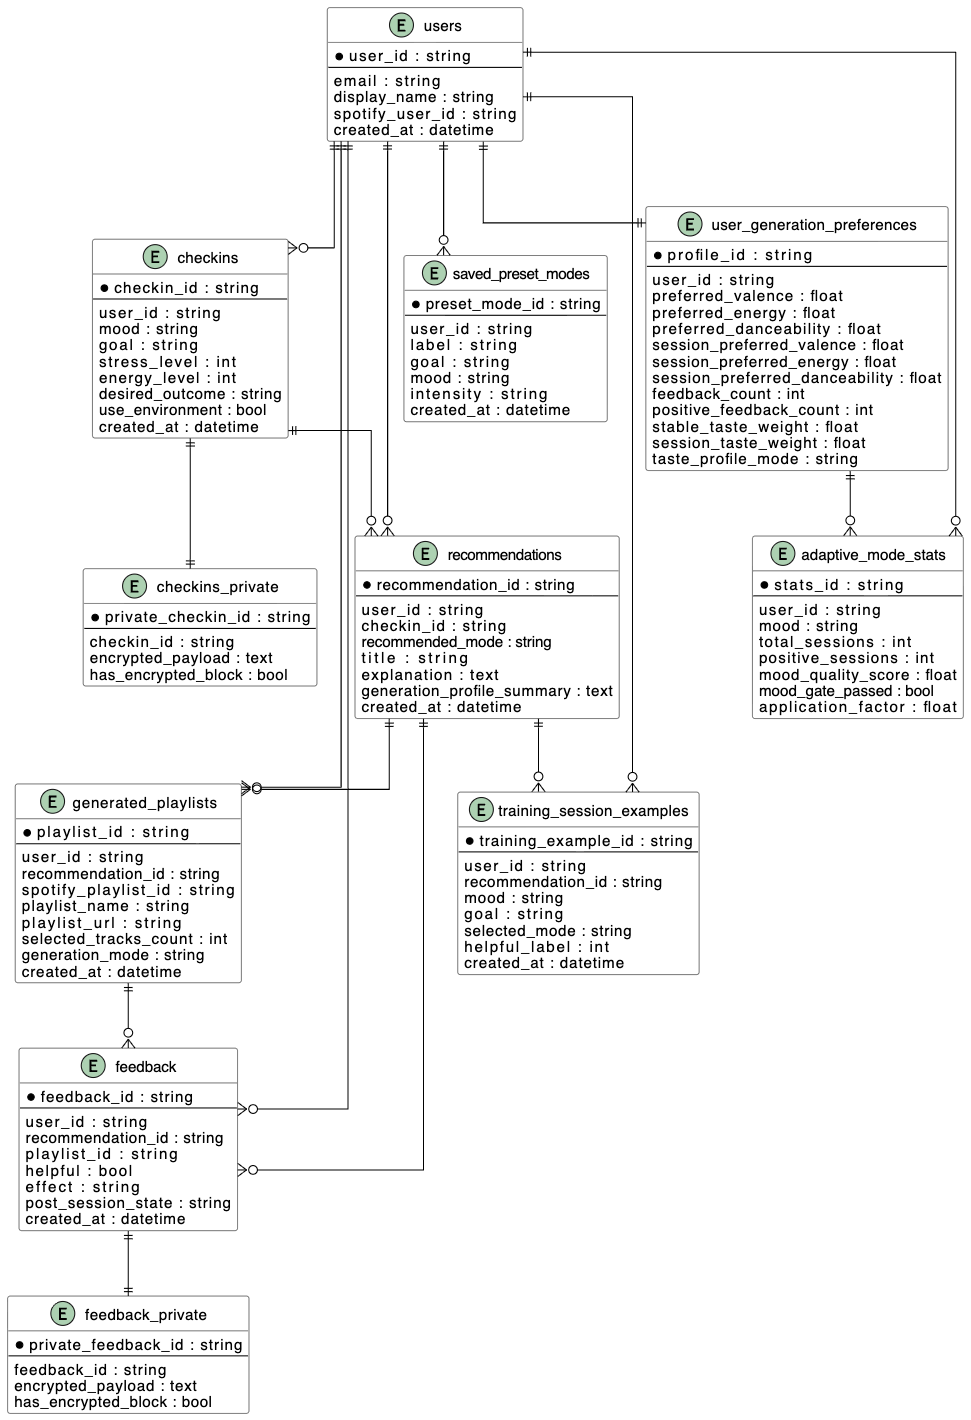
\includegraphics[width=0.78\linewidth]{Imagenes/diagrama_entidad_relacion.png}
    \caption{Diagrama entidad-relación lógico principal de Harmony Hub.}
    \label{fig:er_principal}
\end{figure}

\subsection{Colecciones y documentos principales}

\begin{center}
\captionsetup{type=table}
\scriptsize
\renewcommand{\arraystretch}{1.1}
\setlength{\tabcolsep}{3pt}
\begin{tabularx}{\textwidth}{|P{2.75cm}|P{1.9cm}|Y|P{1.9cm}|}
\hline
\textbf{Colección} & \textbf{ID doc.} & \textbf{Contenido representativo} & \textbf{Nivel} \\
\hline
\texttt{users} & UID del usuario & Perfil mínimo autenticado y referencia de identidad. & Alta \\
\hline
\texttt{checkins} & ID autogenerado & Bloque público mínimo del check-in: usuario, resumen del entorno acústico, densidad de muestreo, estabilidad, referencia al bloque privado y fecha. & Media \\
\hline
\shortstack[l]{\texttt{checkins\_}\\\texttt{private}} & Mismo ID del check-in & Bloque cifrado con estado de ánimo, objetivo, estrés, energía y resultado deseado. & Alta \\
\hline
\shortstack[l]{\texttt{recommendations}} & ID autogenerado & Título de recomendación, modo recomendado, targets musicales, origen de selección, estado de uso del entorno y contexto resumido. & Media \\
\hline
\shortstack[l]{\texttt{generated\_}\\\texttt{playlists}} & ID autogenerado & Identificador y URL de playlist, modo usado, número de pistas, pesos de aprendizaje aplicados y estado final del uso del entorno. & Media \\
\hline
\texttt{feedback} & ID autogenerado & Referencia a la recomendación, uso para aprendizaje, alcance de preferencia y bloque público mínimo. & Media \\
\hline
\shortstack[l]{\texttt{feedback\_}\\\texttt{private}} & Mismo ID del feedback & Valoración global, estado posterior de sesión y comentario cifrado. & Alta \\
\hline
\shortstack[l]{\texttt{saved\_preset\_}\\\texttt{modes}} & UID\_modo & Modo rápido guardado por el usuario y sus metadatos descriptivos. & Baja \\
\hline
\shortstack[l]{\texttt{user\_generation\_}\\\texttt{preferences}} & ID Spotify del usuario & Perfil aprendido agregado: preferencias de energía, valencia, ritmo, pesos estable/contextual y estadísticas específicas por mood. & Media \\
\hline
\shortstack[l]{\texttt{training\_session\_}\\\texttt{examples}} & UUID & Ejemplos agregados de sesión cerrada usados para entrenar y evaluar el modelo supervisado. & Media \\
\hline
\end{tabularx}
\caption{Colecciones principales de Firestore y tipo de información que almacenan.}
\label{tab:colecciones_firestore}
\end{center}

Esta organización muestra una decisión de diseño relevante: las unidades de uso
visibles para el usuario (check-in, recomendación, playlist y feedback) no se
guardan como un único documento gigante, sino como un conjunto trazable de
documentos enlazados. La separación entre bloques públicos mínimos y bloques
privados cifrados reduce exposición innecesaria y, además, mantiene claridad
sobre qué piezas necesita realmente cada parte de la aplicación.

También conviene distinguir dos niveles de agregación que en la interfaz pueden
parecer similares pero no cumplen la misma función. El documento de
preferencias de generación conserva el perfil visible del usuario y contadores
agregados de uso, mientras que la colección de ejemplos de entrenamiento a
nivel de sesión representa la base real utilizada para el modelo supervisado.
Esta separación resulta útil porque el perfil puede mostrar aprendizaje
acumulado y insights válidos aun cuando el clasificador global todavía
no dispone de balance suficiente para activarse.

En el estado actual del proyecto, esta diferencia ya se aprecia con claridad en
la práctica. El perfil visible del usuario longitudinal empleado para la
validación muestra actividad acumulada suficiente para sostener aprendizaje
individual estable, mientras que la base real del modelo supervisado de sesión
continúa condicionada por el balance entre ejemplos útiles y no útiles. Esta
asimetría no es un error de datos, sino la consecuencia de distinguir entre un
perfil agregado de uso visible y el subconjunto de sesiones realmente
consolidado para entrenamiento supervisado.

\section{Diseño funcional}
\label{sec:diseno_funcional}

Desde el punto de vista funcional, la solución se apoya en varios módulos que
cooperan entre sí: autenticación, gestión de sesión con Spotify, captura del
entorno, recomendación, persistencia de historial, gestión del feedback y modos
rápidos.

La \textbf{Figura~\ref{fig:clases_general}} resume esta organización interna a
través de un diagrama de clases general. En él se aprecia cómo la aplicación se
articula alrededor de servicios, modelos y componentes de persistencia
especializados, en lugar de concentrar demasiada lógica en una sola capa.

Además, para comprender bien el comportamiento dinámico del sistema, conviene
observar cómo se encadena el flujo completo de una sesión musical. La
\textbf{Figura~\ref{fig:actividades_sesion}} resume primero esa lógica desde un
punto de vista de actividades y decisiones. A continuación, la
\textbf{Figura~\ref{fig:secuencia_principal}} representa la secuencia principal
desde la interacción inicial del usuario hasta la creación de la playlist y el
registro del feedback posterior.

Este bloque funcional puede leerse desde tres perspectivas complementarias. La
vista de clases ayuda a entender qué piezas cooperan entre sí; la vista de
actividades muestra en qué orden se activan las decisiones principales; y la
vista de secuencia deja ver cómo circulan las llamadas entre cliente, backend,
motor híbrido y servicios externos durante una sesión real.

Por último, el cierre del ciclo se detalla en la
\textbf{Figura~\ref{fig:secuencia_feedback}}, donde se aprecia cómo el feedback
del usuario no solo se almacena, sino que desencadena la actualización del
perfil individual, la conservación de ejemplos supervisados y la auditoría del
estado del modelo.

\begin{landscape}
\begin{figure}[p]
    \centering
    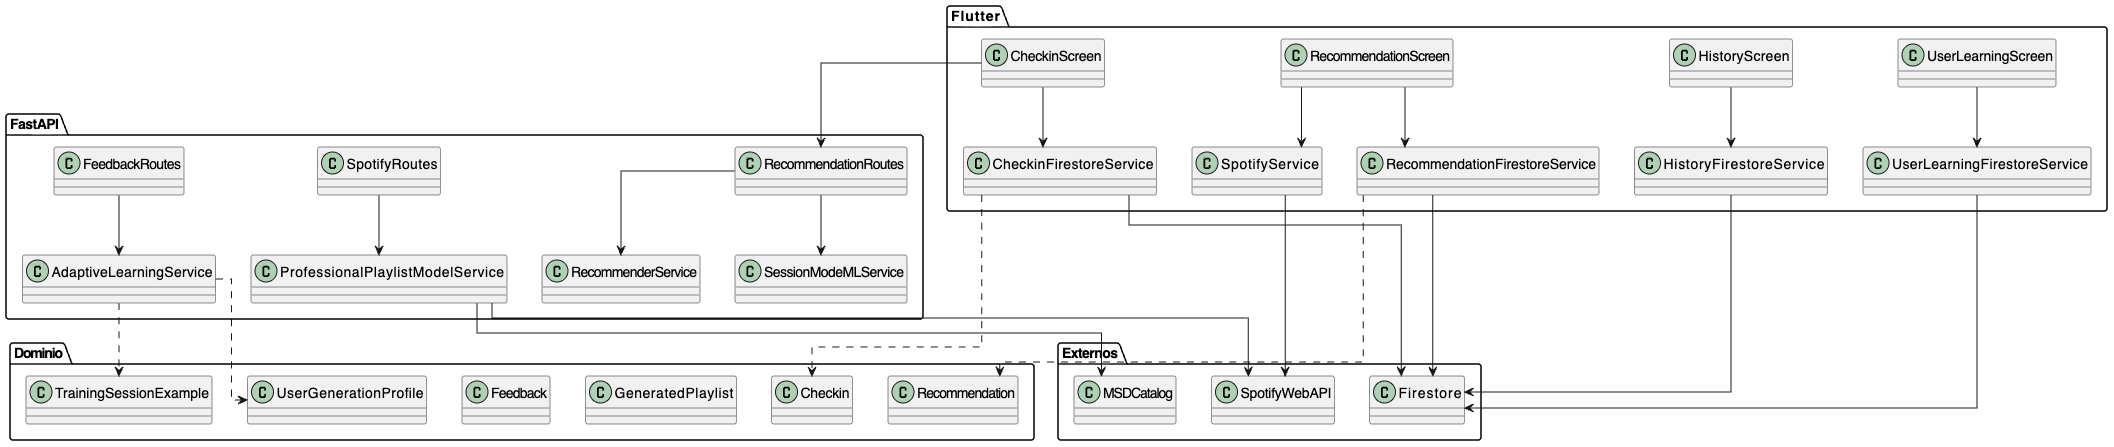
\includegraphics[width=\linewidth,height=0.84\textheight,keepaspectratio]{Imagenes/diagrama_clases_general.png}
    \caption{Diagrama de clases general de Harmony Hub.}
    \label{fig:clases_general}
\end{figure}
\end{landscape}

La vista de actividades permite leer el flujo desde una perspectiva menos
estructural y más operativa. En ella se distinguen con claridad tres momentos:
la recogida del contexto inicial mediante el check-in y, en su caso, el
entorno acústico; la generación y materialización de la sesión musical; y el
cierre del ciclo por medio del feedback, que activa tanto la actualización del
perfil aprendido como la consolidación de nuevos ejemplos supervisados. La
representación también resulta útil para mostrar que ciertos pasos son
condicionales, como la medición del entorno, la solicitud de playlist o el
envío de feedback posterior.

\begin{figure}[H]
    \centering
    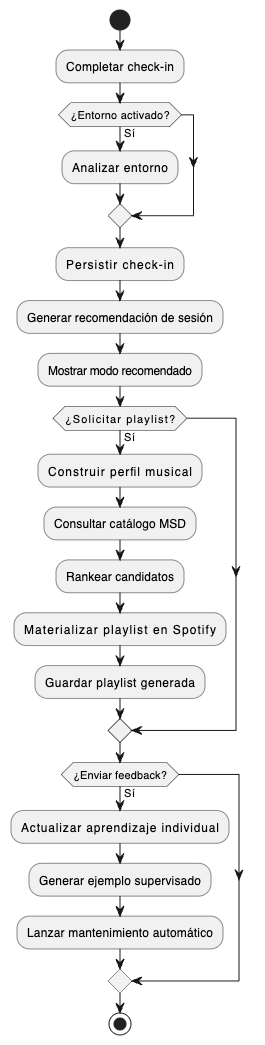
\includegraphics[width=0.38\textwidth,height=0.56\textheight,keepaspectratio]{Imagenes/diagrama_actividades_sesion.png}
    \caption{Diagrama de actividades del flujo principal de generación de sesión musical.}
    \label{fig:actividades_sesion}
\end{figure}

\begin{landscape}
\begin{figure}[p]
    \centering
    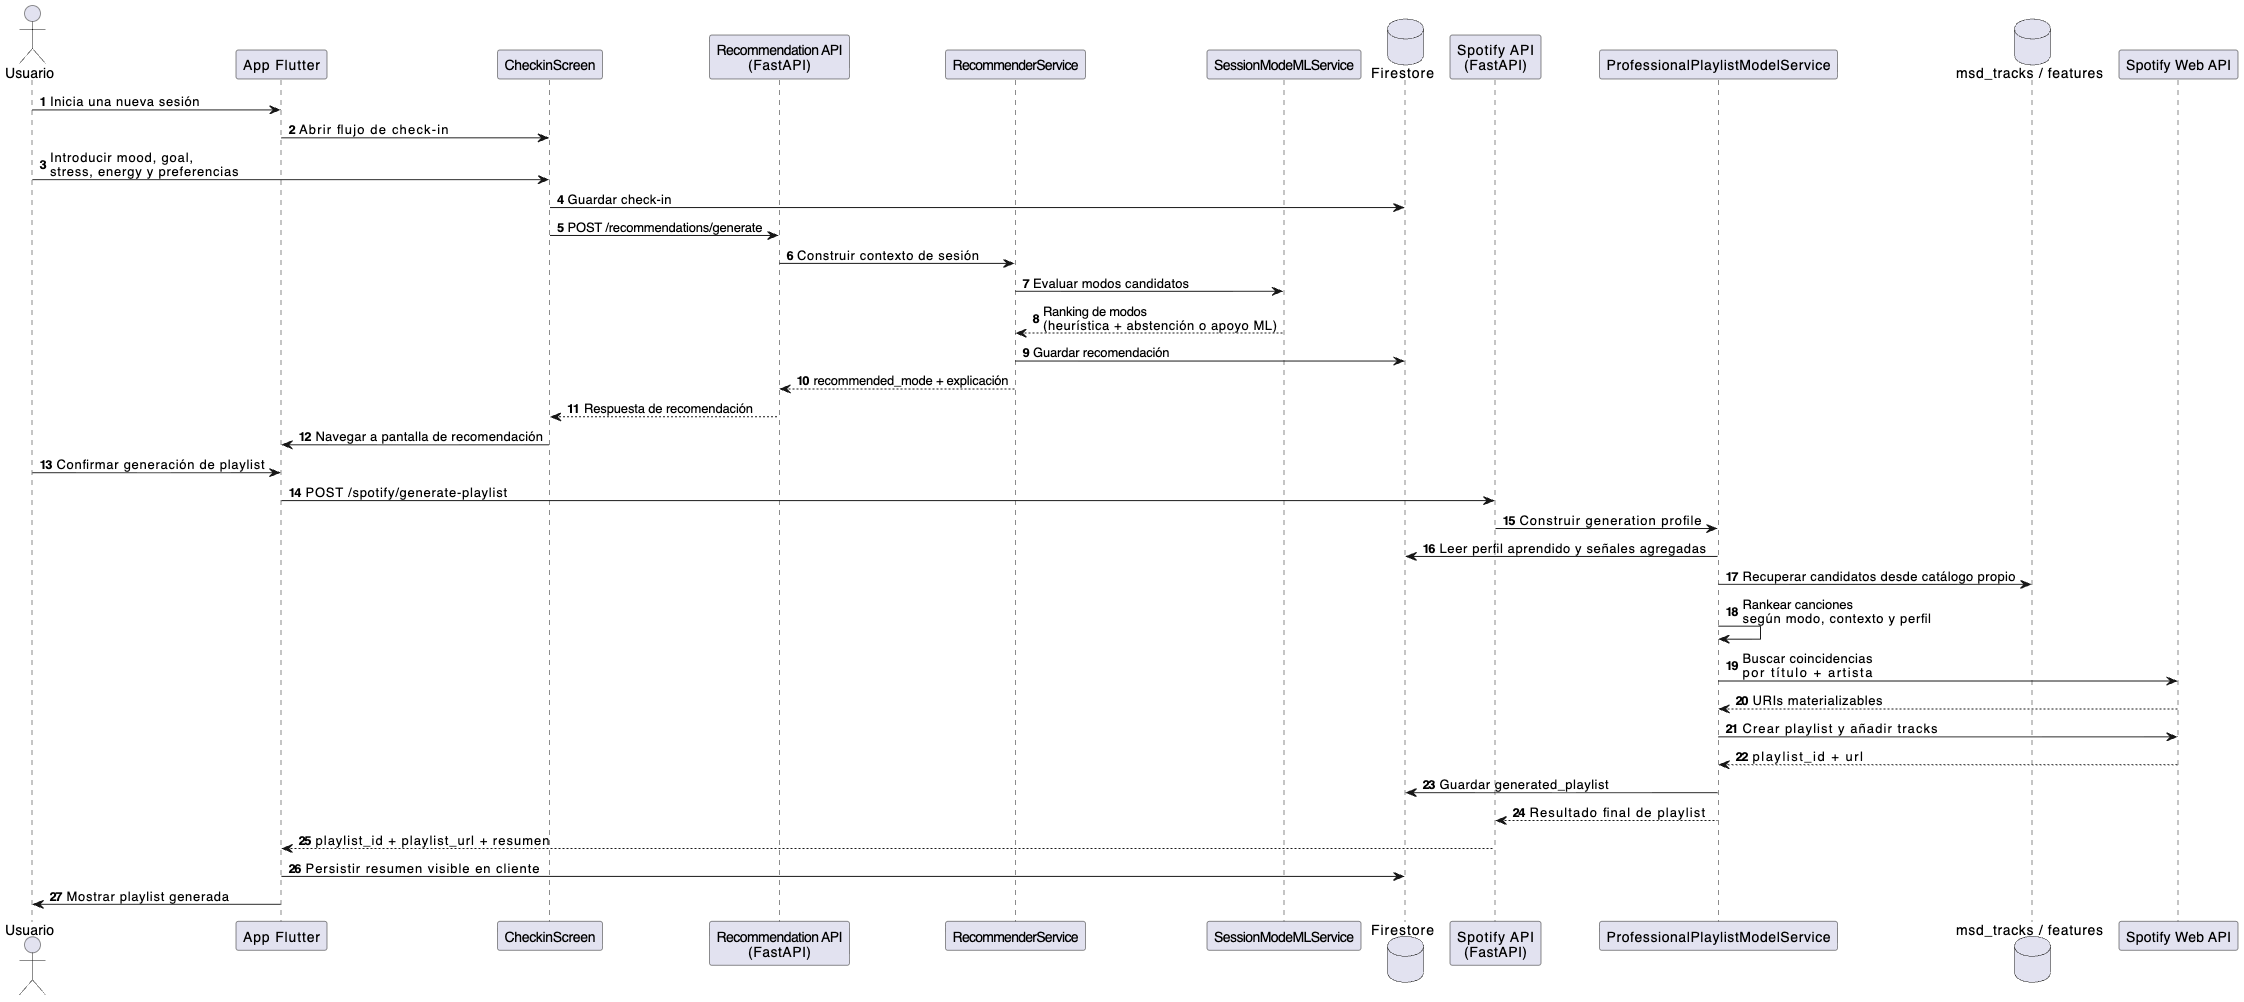
\includegraphics[width=\linewidth,height=0.84\textheight,keepaspectratio]{Imagenes/diagrama_secuencia_principal.png}
    \caption{Diagrama de secuencia principal del flujo de generación de sesión musical.}
    \label{fig:secuencia_principal}
\end{figure}
\end{landscape}

Ese flujo general se complementa con una vista más específica del tratamiento
del feedback. La \textbf{Figura~\ref{fig:secuencia_feedback}} muestra cómo el
backend utiliza esa valoración para actualizar estadísticas, conservar ejemplos
de entrenamiento y, además, separar el feedback público de la parte sensible
cifrada antes de persistirlo en Firestore.

\begin{landscape}
\begin{figure}[p]
    \centering
    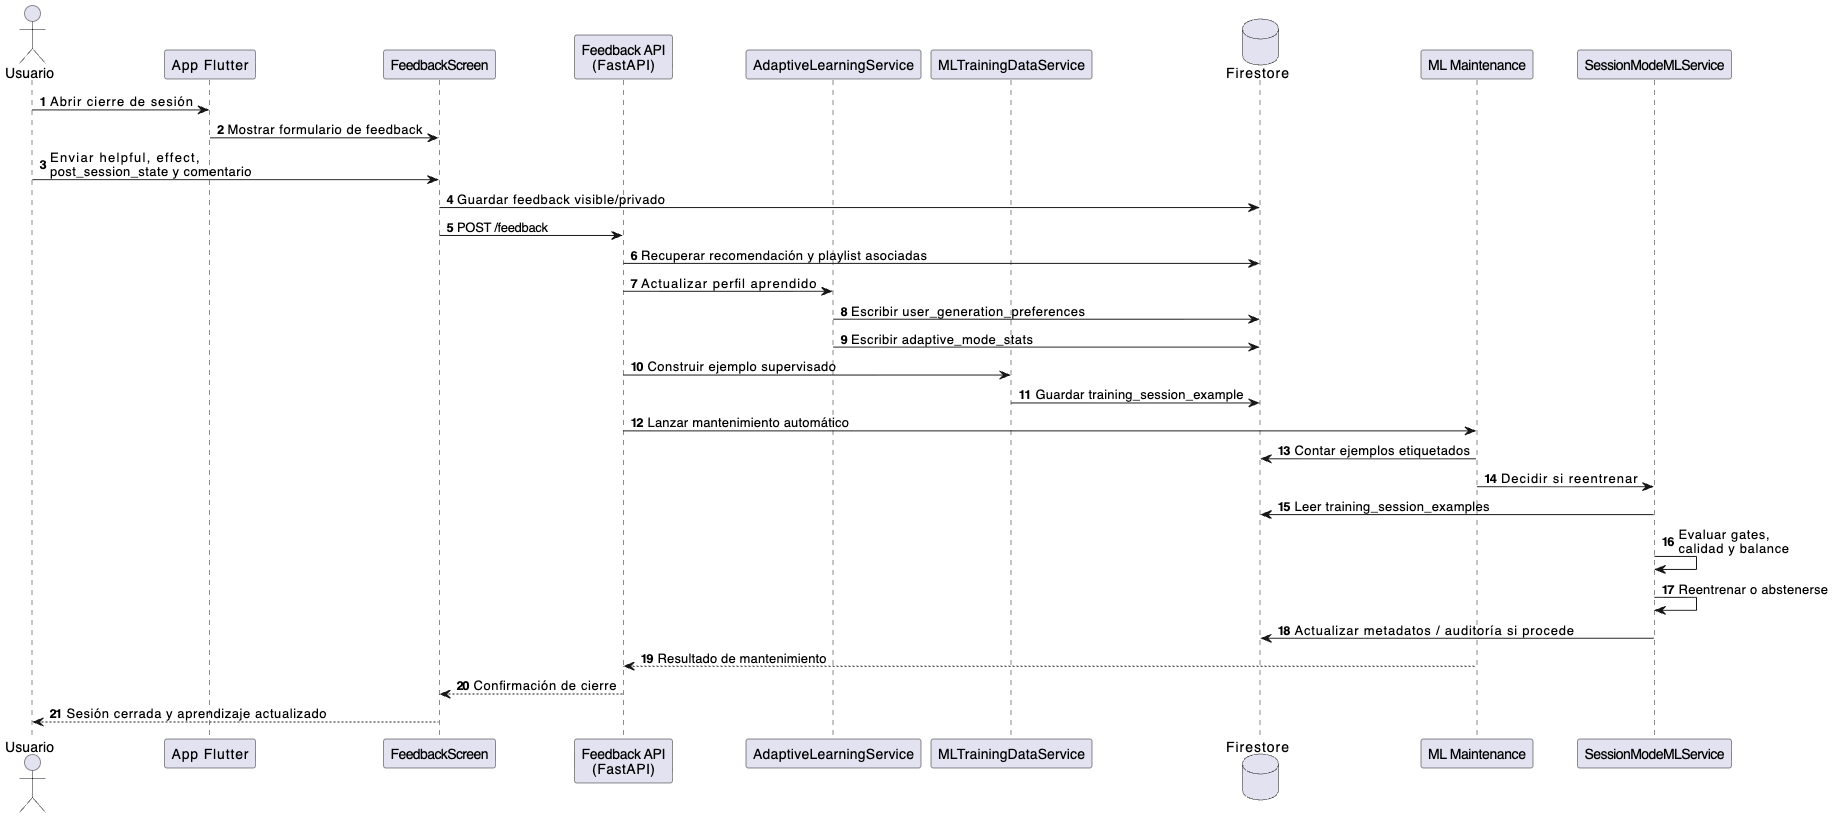
\includegraphics[width=0.92\linewidth,height=0.8\textheight,keepaspectratio]{Imagenes/diagrama_secuencia_feedback.png}
    \caption{Diagrama de secuencia específico del proceso de feedback y actualización del aprendizaje.}
    \label{fig:secuencia_feedback}
\end{figure}
\end{landscape}

La lógica operativa de este cierre puede resumirse en un pseudocódigo breve, en
el que se observa cómo el feedback no solo registra la valoración de la sesión,
sino que desencadena la actualización del perfil individual y la consolidación
de nuevos ejemplos para el modelo supervisado.

\begin{listing}[H]
\begin{minted}[fontsize=\small,breaklines]{text}
ALGORITMO CerrarSesionConFeedback(feedback, recomendacion, playlist)
  guardar bloque publico y bloque privado del feedback
  recuperar contexto de recomendacion y playlist asociada

  actualizar perfil aprendido del usuario
  actualizar estadisticas agregadas por mood

  construir ejemplo supervisado de sesion cerrada
  guardar ejemplo en la coleccion de entrenamiento

  ejecutar mantenimiento automatico del modelo
  SI el reentrenado supera puertas de datos y calidad ENTONCES
    actualizar artefactos y metadatos del modelo
  SI NO
    mantener abstencion conservadora
  FIN SI
FIN ALGORITMO
\end{minted}
\caption{Pseudocódigo del cierre de sesión con feedback y actualización del aprendizaje.}
\label{lst:pseudocodigo_feedback}
\end{listing}

Si se sigue el mismo hilo que aparece en el diagrama general de casos de uso,
el diseño funcional puede entenderse como una cadena de bloques que se apoyan
entre sí y que, poco a poco, van cerrando el ciclo completo de uso.

\subsection{Acceso y recuperación de cuenta}

El primer bloque cubre el alta del usuario, el inicio de sesión y la
recuperación de contraseña. Aunque pueda parecer una parte más convencional del
proyecto, aquí ya aparecen dos necesidades importantes: reducir fricción de
entrada y asegurar que la experiencia no se rompa cuando el usuario pierde el
acceso a la cuenta. Por eso se optó por una autenticación basada en Firebase,
con persistencia mínima del perfil y un mecanismo de restablecimiento que se
apoya en el correo real asociado a la cuenta.

\subsection{Check-in y generación de recomendación}

El núcleo de Harmony Hub empieza realmente en el check-in. Esta parte está
pensada para capturar el estado del usuario sin convertir la interacción en un
formulario pesado. Se recogen variables como estado de ánimo, objetivo, nivel
de energía, nivel de estrés y, cuando procede, contexto acústico del entorno.

Después, el backend traduce ese contexto en una recomendación de sesión. Aquí
la intención no es decirle al usuario ``qué canción debería escuchar'', sino
darle una propuesta funcional de sesión con sentido para ese momento concreto.
Además, cada recomendación queda vinculada a un identificador que sirve como
hilo conductor del resto del flujo.

\subsection{Conexión con Spotify y materialización de la sesión}

La recomendación, por sí sola, todavía no resuelve el problema. Tiene que
convertirse en una playlist real y reproducible dentro de una plataforma de uso
cotidiano. Para eso se integra Spotify mediante OAuth y un backend intermedio
que gestiona tanto el intercambio de credenciales como la creación posterior de
la playlist.

Este bloque tiene bastante peso arquitectónico, porque conecta el dominio
propio de Harmony Hub con un servicio externo sobre el que la aplicación no
tiene control absoluto. Y es precisamente ahí donde cobra sentido haber
separado interfaz, backend y persistencia.

\subsection{Historial y memoria de uso}

Una vez generadas varias sesiones, la aplicación necesita ofrecer al usuario un
espacio donde recuperar lo vivido. El historial no se plantea solo como una
lista de eventos técnicos, sino como una memoria funcional de check-ins,
recomendaciones, playlists y valoraciones. Esto permite volver sobre sesiones
anteriores, reinterpretar patrones y reforzar la sensación de continuidad entre
usos.

\subsection{Modos rápidos}

Los modos rápidos responden a una idea bastante simple, pero muy útil: hay
situaciones que se repiten. Por eso el sistema ofrece accesos predefinidos para
momentos como entrar en foco, bajar carga mental o cambiar de ritmo tras una
jornada intensa. Desde el diseño funcional, esta capa actúa como un atajo
práctico entre el uso libre y el uso recurrente.

\subsection{Feedback y aprendizaje personal}

El cierre del flujo llega con el feedback. Cuando el usuario valora si la
sesión le ayudó, la aplicación no solo guarda una respuesta; convierte esa
valoración en evidencia para entender mejor qué propuestas funcionan y cuáles
no. Además, este diseño se ha construido con una separación entre bloque
público y bloque privado cifrado, algo que refuerza la seguridad de información
sensible como comentarios o estados posteriores de sesión.

Por encima de ese feedback puntual aparece el aprendizaje personal, que no se
presenta como una inteligencia mágica ni como una caja negra opaca. Se apoya en
estadísticas acumuladas, trazabilidad entre recomendación y resultado, y una
aplicación prudente de pesos aprendidos. En la implementación actual esto se traduce en
modos operativos como \texttt{progressive\_contextual} o
\texttt{stable\_weighted}, que permiten explicar cuándo el sistema usa memoria
estable, cuándo aplica solo una parte de lo aprendido y cuándo todavía depende
principalmente del contexto inmediato.

En la práctica, esta capa es también la que alimenta la pantalla de aprendizaje
visible para el usuario. Los insights sobre tono emocional, energía o
ritmo habitual se derivan del documento agregado del perfil, no del artefacto
del modelo supervisado. Esto mejora la explicabilidad del producto final,
porque permite enseñar aprendizaje útil incluso cuando el clasificador global
todavía no ha alcanzado madurez suficiente.

Conviene precisar cómo decide el sistema si una sesión debe apoyarse más en el
perfil reciente o en el perfil estable. En la implementación actual se calculan
dos pesos continuos: un peso de sesión, asociado a la evidencia contextual o
de corto plazo, y un peso estable, asociado al histórico más consolidado del
usuario. Ambos pesos no se fijan manualmente, sino que dependen de la
consistencia observada en el feedback positivo y negativo acumulado. Cuando el
peso estable supera al peso de sesión, el modo interno del perfil pasa a
\texttt{stable\_weighted}; cuando ocurre lo contrario, el sistema utiliza
\texttt{session\_weighted}. Si la evidencia del mood actual todavía no es
suficiente para aplicar el aprendizaje completo, aparece un estado intermedio,
\texttt{progressive\_contextual}, que mantiene una aplicación parcial y más
prudente.

Este reparto se normaliza reservando una masa base unitaria para el contexto
actual de la sesión. La decisión no es arbitraria: sirve para garantizar que
el aprendizaje previo no sustituya el check-in presente, sino que actúe como
factor de corrección progresiva. En otras palabras, el sistema preserva un
espacio fijo para lo que el usuario declara y vive en ese momento —objetivo,
estado emocional, nivel de energía, estrés, resultado deseado y entorno—, y
solo después distribuye el peso adicional entre memoria de sesión y memoria
estable según la evidencia observada. Gracias a esta masa base, Harmony Hub
aprende sin encasillar y mantiene la capacidad de responder principalmente a la
necesidad del momento.

El efecto real de esta decisión no consiste en sustituir el check-in por el
histórico, sino en desplazar progresivamente los valores objetivo de la
sesión. Por ejemplo, si el contexto actual sugiere una energía base de 0.50,
el aprendizaje reciente de sesión apunta a 0.44 y el perfil estable indica que
históricamente suele funcionar mejor una energía próxima a 0.38, el sistema no
salta directamente al valor estable. Primero mezcla el valor base con el valor
de sesión según su peso contextual y, después, vuelve a mezclar el resultado
con el valor estable. Si, por ejemplo, el peso de sesión es 0.17 y el peso
estable es 0.28, el valor final de energía queda aproximadamente en 0.46. Esto
permite conservar la señal del momento actual, pero corrigiéndola de forma
gradual hacia lo que el histórico del usuario ha demostrado que suele
funcionarle mejor. La misma lógica se aplica también a los valores objetivo de
valencia y bailabilidad, por lo que la diferencia entre un perfil más estable y
uno más contextual se traduce en ajustes musicales reales, no solo en una
etiqueta mostrada en pantalla.

La Tabla~\ref{tab:modos_perfil_aprendizaje} resume de forma comparativa estos
cuatro estados internos del perfil aprendido y su efecto práctico sobre la
sesión.

\begin{table}[H]
\centering
\small
\renewcommand{\arraystretch}{1.12}
\begin{tabularx}{\textwidth}{|P{2.9cm}|P{3.1cm}|Y|}
\hline
\textbf{Modo interno} & \textbf{Condición principal} & \textbf{Interpretación funcional} \\
\hline
\texttt{\seqsplit{context\_only}} & La suma de pesos aprendidos es prácticamente nula. & El sistema trabaja casi exclusivamente con el check-in actual. Todavía no existe evidencia suficiente como para que el aprendizaje previo modifique de forma apreciable los targets musicales. \\
\hline
\texttt{\seqsplit{progressive\_contextual}} & El mood actual aún no ha superado su umbral de madurez local, pero ya existe cierta evidencia parcial. & Se aplica una parte del aprendizaje acumulado de forma prudente. El sistema no ignora el histórico, pero evita dejar que domine mientras la evidencia específica del mood siga siendo insuficiente. \\
\hline
\texttt{\seqsplit{session\_weighted}} & El peso de sesión es mayor o igual que el peso estable. & La sesión se corrige principalmente con señales recientes o más contextuales. Esto suele ocurrir cuando el patrón observado en sesiones próximas resulta más informativo que el histórico general. \\
\hline
\texttt{\seqsplit{stable\_weighted}} & El peso estable supera al peso de sesión. & La corrección principal proviene del perfil histórico consolidado. El sistema sigue partiendo del check-in actual, pero desplaza con más fuerza los targets hacia aquello que ha demostrado funcionar mejor de forma recurrente para el usuario. \\
\hline
\end{tabularx}
\caption{Estados internos del perfil aprendido y su efecto sobre la personalización musical.}
\label{tab:modos_perfil_aprendizaje}
\end{table}

\section{Diseño de la interfaz}
\label{sec:diseno_interfaz}

La interfaz se diseñó con una idea bastante clara desde el principio: la app
debía sentirse íntima, ligera y guiada, no como una herramienta técnica que
obliga al usuario a pensar demasiado antes de poder usarla. Y es que, si el
objetivo del sistema es ayudar a regular un momento interno, una interfaz fría
o excesivamente mecánica jugaría en contra de esa intención.

En términos de navegación, la aplicación se estructura alrededor de una barra
inferior con accesos a los apartados principales: inicio, modos, historial,
aprendizaje y perfil. Esta organización busca que el usuario tenga siempre una
idea bastante clara de dónde está y qué puede hacer a continuación.

La Figura~\ref{fig:diagrama_navegacion_app} resume este recorrido de manera
global. En ella se observa tanto el acceso inicial mediante autenticación y
conexión con Spotify como la navegación principal dentro del \textit{AppShell},
desde donde se articula el flujo más importante del sistema: check-in,
recomendación, generación de playlist y devolución de feedback.

\begin{figure}[htbp]
\centering
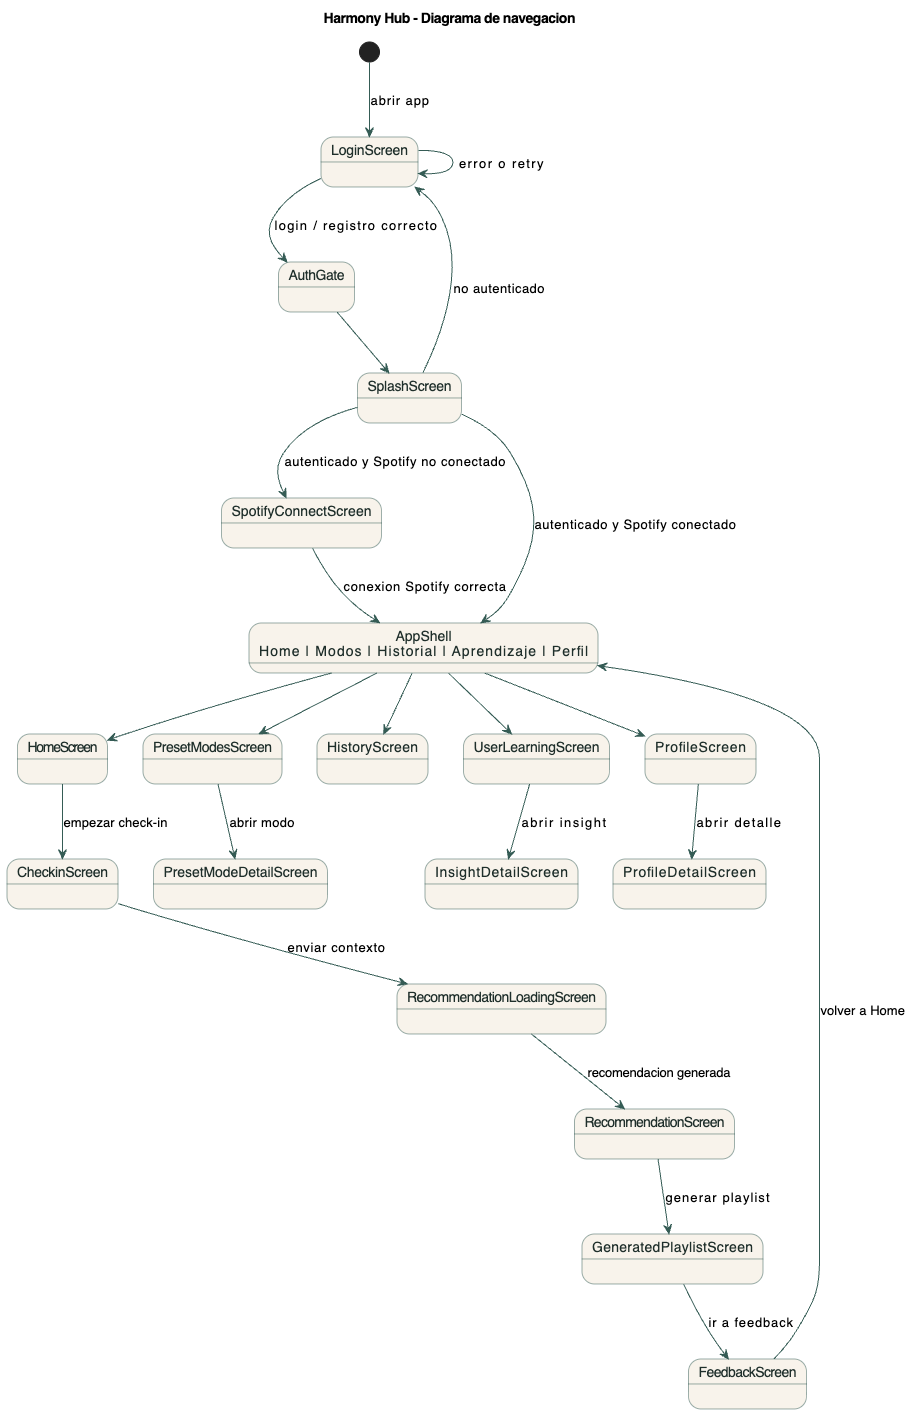
\includegraphics[width=0.72\textwidth]{Imagenes/diagrama_navegacion_app.png}
\caption{Diagrama de navegación principal de Harmony Hub.}
\label{fig:diagrama_navegacion_app}
\end{figure}

Para complementar esa visión estructural, resulta útil mostrar también algunas
pantallas clave del producto final. La Figura~\ref{fig:interfaz_principal_app}
reúne cuatro momentos representativos del flujo: acceso inicial, pantalla
principal, recomendación contextual y playlist generada. Esta selección permite
ver cómo la lógica funcional del sistema se traduce en una interfaz móvil
coherente y suficientemente guiada.

\begin{figure}[htbp]
\centering
\begin{minipage}{0.23\textwidth}
    \centering
    
\includegraphics[width=\linewidth]{Imagenes/manual_app/Screenshot_2026-05-25-18-37-08-051_com.example.harmonyhub.jpg}
\end{minipage}
\hfill
\begin{minipage}{0.23\textwidth}
    \centering
    
\includegraphics[width=\linewidth]{Imagenes/manual_app/Screenshot_2026-05-25-18-46-14-698_com.example.harmonyhub.jpg}
\end{minipage}
\hfill
\begin{minipage}{0.23\textwidth}
    \centering
    
\includegraphics[width=\linewidth]{Imagenes/manual_app/Screenshot_2026-05-25-18-49-39-980_com.example.harmonyhub.jpg}
\end{minipage}
\hfill
\begin{minipage}{0.23\textwidth}
    \centering
    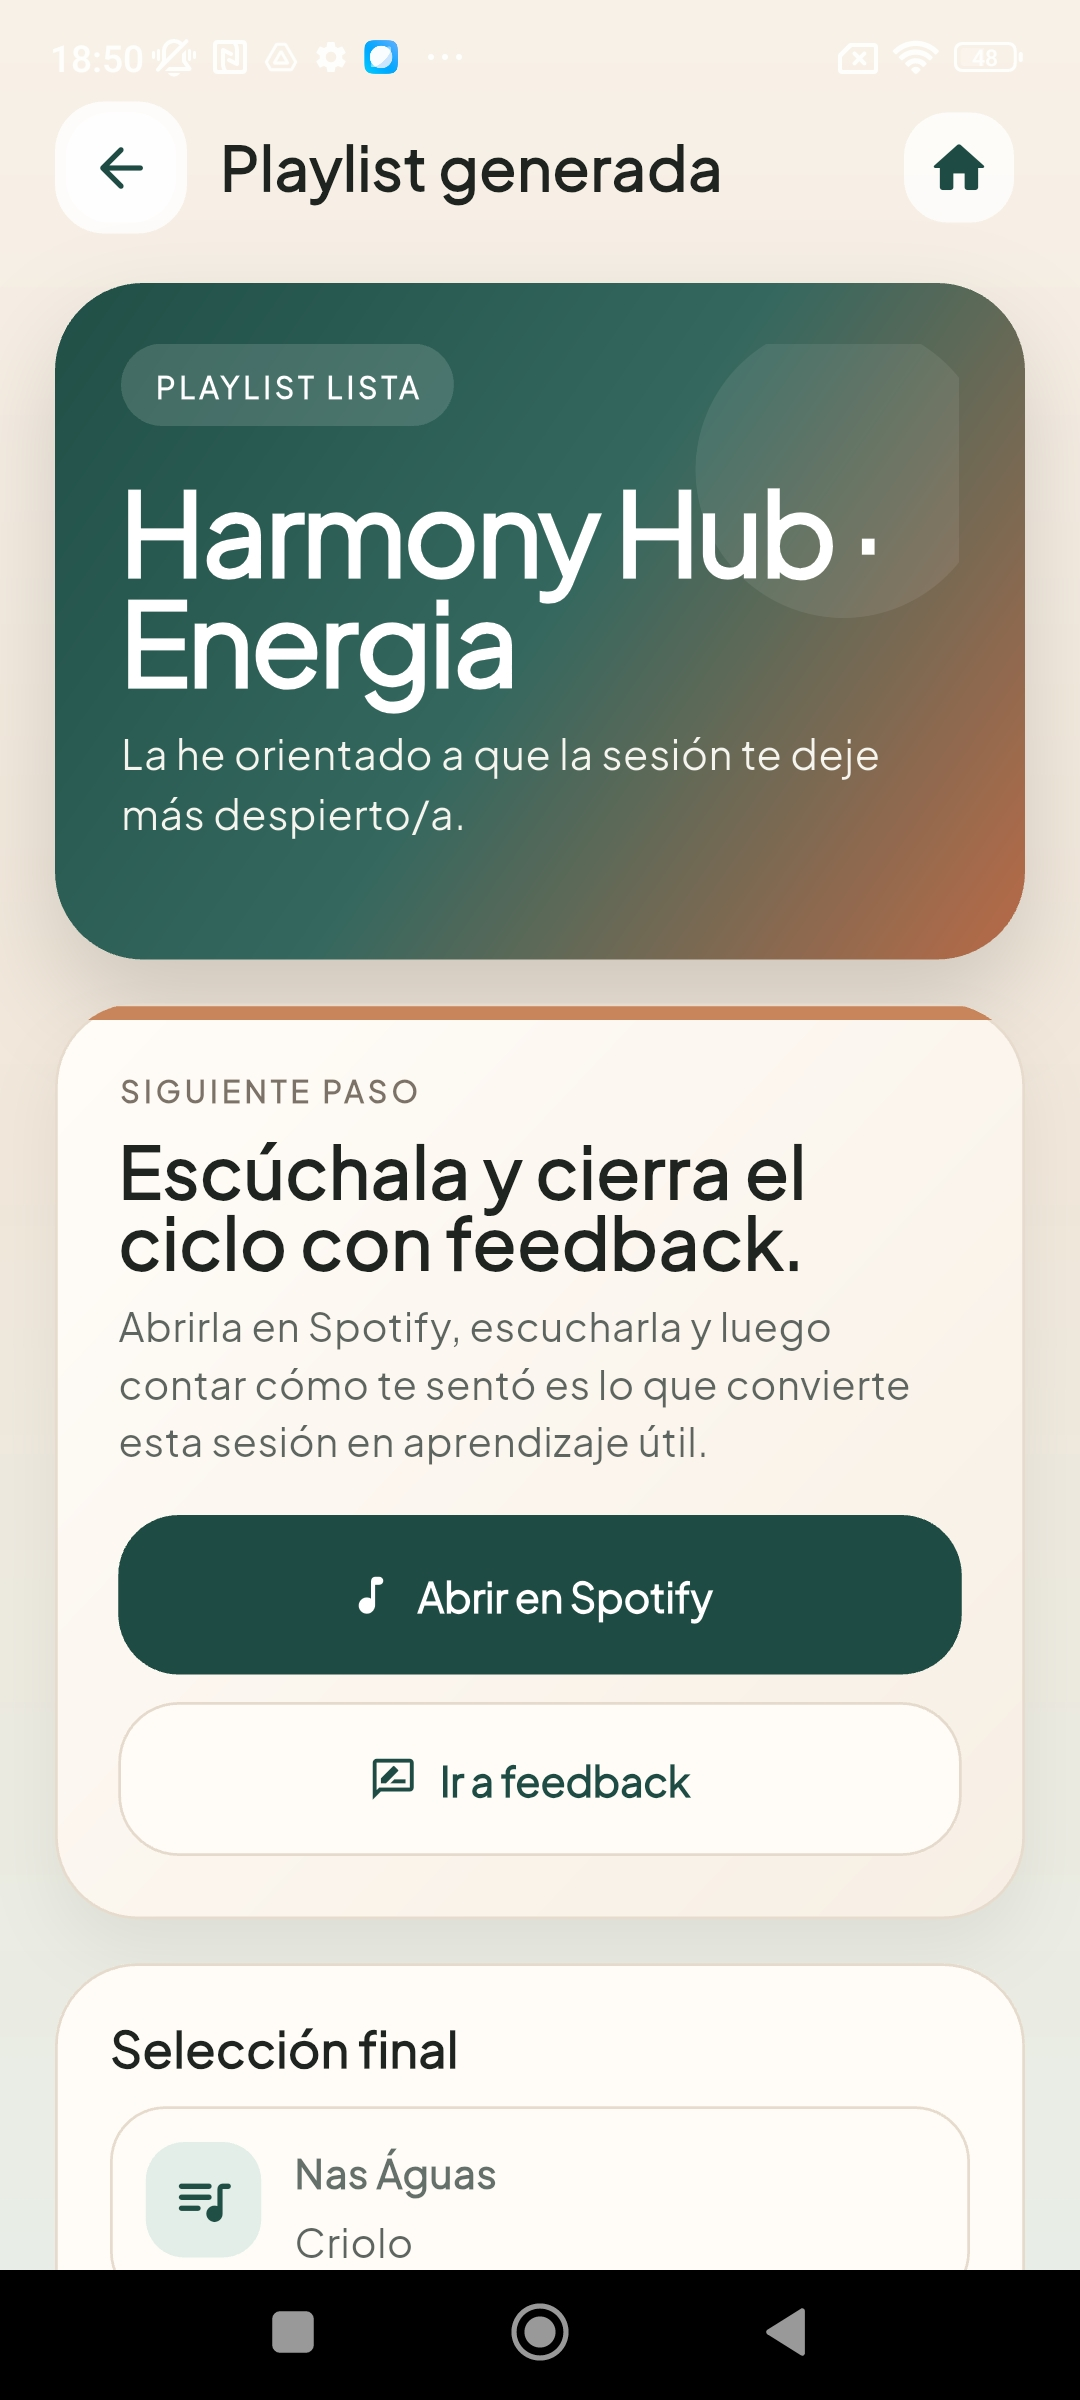
\includegraphics[width=\linewidth]{Imagenes/manual_app/Screenshot_2026-05-25-18-50-27-942_com.example.harmonyhub.jpg}
\end{minipage}
\caption{Pantallas representativas de la interfaz final: acceso, inicio, recomendación y playlist generada.}
\label{fig:interfaz_principal_app}
\end{figure}

Estas capturas permiten identificar cuatro decisiones de diseño. En primer
lugar, el acceso utiliza una jerarquía visual suave y directa, evitando
sobrecargar la pantalla inicial. En segundo lugar, la pantalla principal
prioriza la acción inmediata de comenzar una nueva sesión, lo que refuerza la
naturaleza cotidiana del uso. En tercer lugar, la recomendación no se presenta
como una simple lista de canciones, sino como una explicación funcional del
tipo de sesión propuesto. Por último, la materialización de la playlist deja
una sensación clara de cierre del flujo, ya que transforma la recomendación en
un recurso reproducible dentro de Spotify.

Desde el punto de vista visual, predominan bloques amplios, esquinas redondeadas,
colores suaves y una jerarquía tipográfica marcada, sobre todo en las pantallas
de acceso, home, Spotify Connect y feedback. No se trata solo de una decisión
estética: ese lenguaje visual ayuda a reducir saturación y refuerza la idea de
acompañamiento en lugar de exigir una interacción áspera o demasiado funcional.

También se tomaron decisiones específicas para mejorar la experiencia en móvil:

\begin{table}[H]
\centering
\small
\renewcommand{\arraystretch}{1.1}
\begin{tabularx}{\textwidth}{|P{4.4cm}|Y|}
\hline
\textbf{Decisión de interfaz} & \textbf{Justificación} \\
\hline
Jerarquía tipográfica muy marcada en pantallas clave & Permite que el usuario entienda rápidamente dónde está y cuál es la siguiente acción importante sin leer bloques largos. \\
\hline
Check-in guiado por pasos cortos & Reduce la sensación de cuestionario y favorece respuestas rápidas en momentos de carga mental o poco tiempo disponible. \\
\hline
CTA principal único por pantalla & Evita competencia entre acciones y refuerza la continuidad del flujo: entrar, responder, preparar playlist, escuchar y dar feedback. \\
\hline
Barra inferior estable para navegación principal & Mantiene orientación constante entre Home, Modos, Historial, Aprendizaje y Perfil, evitando menús escondidos o recorridos ambiguos. \\
\hline
Uso de tarjetas amplias y bloques redondeados & Favorece una percepción más suave y cercana, coherente con el propósito de bienestar cotidiano de la aplicación. \\
\hline
Reducción de densidad textual y agrupación por contexto & Facilita el escaneo rápido y evita saturar la pantalla con explicaciones técnicas o datos redundantes. \\
\hline
Revisión explícita de espaciados y overflows & Resulta necesaria para que la experiencia sea sólida también en dispositivos compactos y no se rompa en momentos críticos del flujo. \\
\hline
Presencia de branding propio y lenguaje visual coherente & Refuerza identidad de producto y ayuda a que Harmony Hub no se perciba como una demo técnica sin personalidad. \\
\hline
\end{tabularx}
\caption{Decisiones específicas adoptadas en el diseño de la interfaz.}
\label{tab:decisiones_interfaz}
\end{table}

\section{Diseño de pruebas}
\label{sec:diseno_pruebas}

El diseño de pruebas se planteó desde una lógica bastante práctica: no bastaba
con comprobar que la app ``abre'' o que una pantalla ``se ve''. Había que
validar el flujo completo, desde el acceso hasta la creación de la playlist y
el almacenamiento del feedback, sin perder de vista el comportamiento del
backend ni la dependencia de servicios externos.

Por eso, las pruebas se estructuran en varios niveles:

\begin{itemize}
    \item pruebas funcionales del flujo principal, centradas en autenticación, check-in, recomendación, playlist, historial y feedback;
    \item pruebas de integración, especialmente en la comunicación entre Flutter, FastAPI, Spotify y Firestore;
    \item pruebas de robustez frente a errores externos, como restricciones o respuestas inesperadas de Spotify;
    \item pruebas de consistencia del aprendizaje, verificando que la información necesaria queda registrada y que el modelo solo se activa con suficiente evidencia;
    \item pruebas de interfaz y usabilidad básica en móvil, incluyendo revisión de overflows, jerarquía visual y continuidad del flujo.
\end{itemize}

Los criterios de aceptación se apoyan en una idea sencilla: cada sesión debe
ser trazable de principio a fin, el sistema debe poder degradarse con dignidad
si falla una parte externa, y la experiencia no debe romperse ni volverse
confusa en un uso cotidiano.

\section{Decisiones técnicas justificadas}
\label{sec:decisiones_tecnicas}

Algunas decisiones técnicas del proyecto no responden solo a disponibilidad de
herramientas, sino al tipo de problema que se quería resolver.

En primer lugar, Flutter permitió construir una experiencia móvil bastante
cuidada y rápida de iterar. Para un TFG con mucho peso en interacción y diseño
de flujo, esa capacidad de probar, ajustar y refinar pantallas en poco tiempo
ha sido especialmente valiosa.

En segundo lugar, FastAPI resultó una opción muy razonable para el backend,
porque facilita exponer endpoints claros, organizar la lógica de recomendación
y mantener separada la parte de cliente respecto a la generación de sesiones y
la integración con Spotify.

La elección de Firestore también responde a una lógica concreta. El proyecto no
necesitaba un modelo relacional estricto, sino una persistencia documental
flexible que permitiera almacenar sesiones, históricos, preferencias y ejemplos
de entrenamiento sin forzar migraciones complejas desde fases tempranas. Además,
encaja bien con estructuras públicas y privadas separadas.

Respecto a Spotify, la integración no se concibe como un simple adorno, sino
como una condición clave de utilidad real. La recomendación de Harmony Hub solo
tiene valor práctico si puede traducirse a una escucha auténtica dentro de una
plataforma que el usuario ya utiliza en su día a día.

Por último, el componente de aprendizaje se ha diseñado con prudencia. En vez
de forzar un modelo activo desde el principio, se ha preferido mantener una
heurística funcional y permitir que el aprendizaje entre solo cuando exista
evidencia suficiente y balanceada. La verdad es que esta decisión sacrifica
algo de espectacularidad aparente, pero gana bastante en honestidad técnica y
fiabilidad del sistema.
